\documentclass[11pt,english]{beamer}
\usepackage{hyperref}
\usepackage{fontawesome}
\usepackage{graphicx}
\usepackage{fontawesome}
\usepackage{FiraSans} 
\usepackage{cancel}
\usepackage[spanish,mexico]{babel}
\usepackage{amsmath}
\usepackage{amsfonts}
\usepackage{amssymb}
\usepackage[square]{natbib}


% Setup appearance:

\usetheme{Darmstadt}
\usefonttheme[onlylarge]{structurebold}
\setbeamerfont*{frametitle}{size=\normalsize,series=\bfseries}
\setbeamertemplate{navigation symbols}{}


% Standard packages

\usepackage[spanish]{babel}
\usepackage[latin1]{inputenc}
\usepackage{times}
\usepackage[T1]{fontenc}


% Setup TikZ

\usepackage{tikz}
\usetikzlibrary{arrows}
\tikzstyle{block}=[draw opacity=0.7,line width=1.4cm]


% Author, Title, etc.

\title[Title] 
{%
Estudios de simulaci�n en la b�squeda de nuevos bosones ligeros durante la fase de alta luminosidad del experimento CMS del CERN %
}

\institute{
\textbf{Autor: }

Lic. Francisco Mart�nez S�nchez\\[.2cm]

\textbf{Miembros del comit�:}


Alfredo Mart�n Casta�eda Hernandez (Director)

Susana Alvarez Garcia (tutor)

Marcelino Barbosa Flores (tutor)

Reporte Avance de Tesis, Universidad de Sonora, Hermosillo, Sonora 2020
}
\date{1 Junio 2020}


% The main document

\begin{document}

\begin{frame}
  \titlepage
\end{frame}

\begin{frame}{Outline}
  \tableofcontents
\end{frame}


\section{Introduccion}

\begin{frame}{}
    \begin{center}
        \LARGE Introducci\'on y Marco Te\'orico
    \end{center}
\end{frame}

\begin{frame}{Evidencias de materia oscura.}
\begin{figure}
\centering
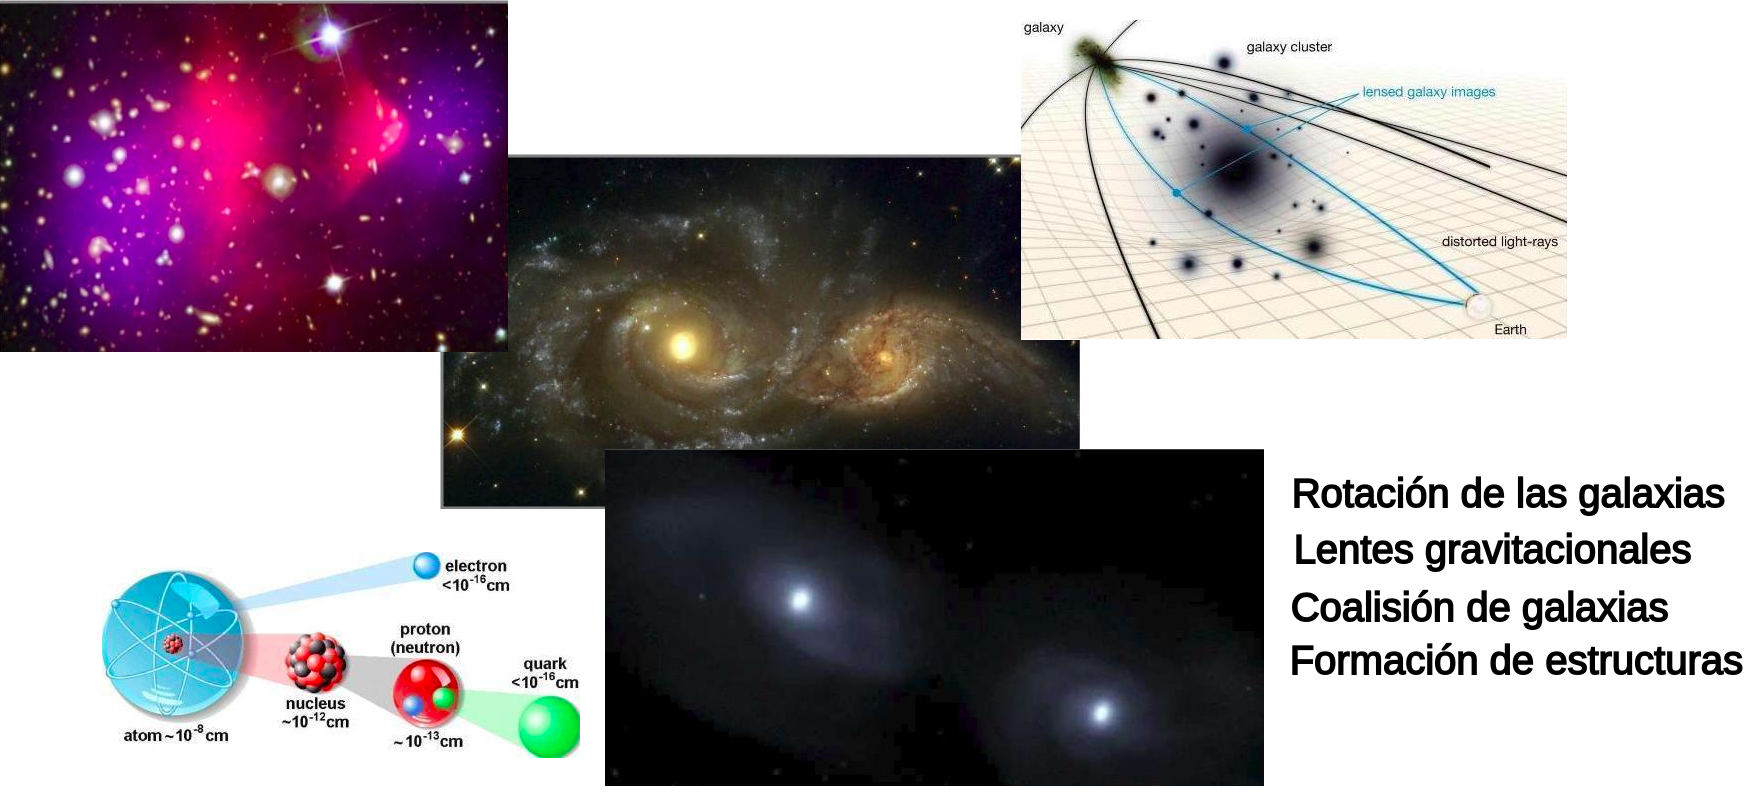
\includegraphics[width=1\textwidth]{Imag/materia_oscura.png}
\end{figure}

\end{frame}


% Teoria que describe la materia bariónica
\begin{frame}{Modelo Est\'andar}

\begin{figure}
\centering
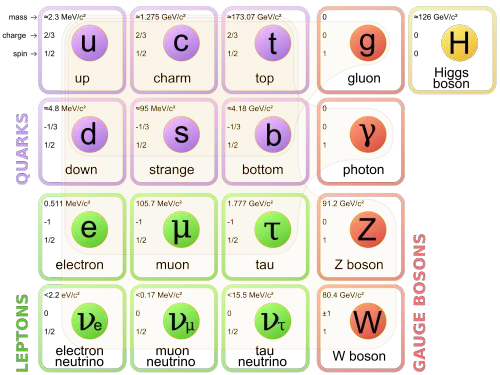
\includegraphics[width=.6\textwidth]{Imag/standard_model.png}
\caption{Modelo est\'andar de la f\'isica de las part\'iculas elementales.}
\end{figure}


\end{frame}



% Teoria que describe la materia bariónica
\begin{frame}{Modelo Est\'andar. Lagrangiano.}

\begin{columns}
\begin{column}{0.35\textwidth}
\Large{
\begin{align*}
\mathcal{L} &= - \frac{1}{4} F_{\mu \nu} F^{\mu \nu} \\
    &\phantom{{}=}+ i \bar{\psi} \cancel{D} \psi + h.c. \\
    &\phantom{{}=}+ \bar{\psi}_i y_{ij} \psi_j \phi + h.c. \\
    &\phantom{{}=}+ |D_\mu \phi|^2 - V(\phi)
\end{align*}
}
\end{column}
\begin{column}{0.65\textwidth}  %%<--- here
    \begin{itemize}
        \item Primera linea describe las fuerzas elementales electromagnetismo, fuerza nuclear debil y fuerte)
        \item La segunda linea describe como las fuerzas actu\'an en las particulas fundamentales (quarks y leptones)
        \item Tercera linea describe como las particulas obtienen sus masas del bos\'on de Higgs 
        \item La cuarta linea describe el campo de Higgs
    \end{itemize}
\end{column}
\end{columns}
\end{frame}


\begin{frame}{Mas alla del modelo est\'andar}

El modelo est\'andar describe de forma exitosa como funciona el universo sin embargo falla en dar explicaci\'on a fen\'omenos tales como:

\begin{itemize}
    \item Descripci\'on cuantica de la fuerza de gravedad
    \item \textbf{Materia Oscura: Por observaciones cosmologicas se sabe que el modelo est\'andar solo contempla el 5\% de la energia presente en el universo.  Cerca de 26\% debe de ser materia oscura, la cual solo interactua debilmente con los campos del modelo est\'andar. El modelo est\'andar no contempla particulas fundamentales como constituyentes de la materia oscura}
    \item Energia Oscura
    \item Masa del neutrino
    \item Asimetria materia-Antimateria
\end{itemize}
    
\end{frame}



\begin{frame}{Mas alla del modelo est\'andar. Modelo Dark-SUSY.}

\begin{itemize}
\item La materia oscura esta compuesta de particulas fundamentales 
\item Estas particulas estan descritas por un formalismo te\'orico parecido al del modelo est\'andar (Teoria cu\'antica de campo) 
\item Que estas nuevas particulas puedan ser producidas por medio de la colisi\'on de protones altamente energ\'eticos (como las producidas en el Gran Acelerador de Hadrones)
\end{itemize}

\begin{figure}
\centering
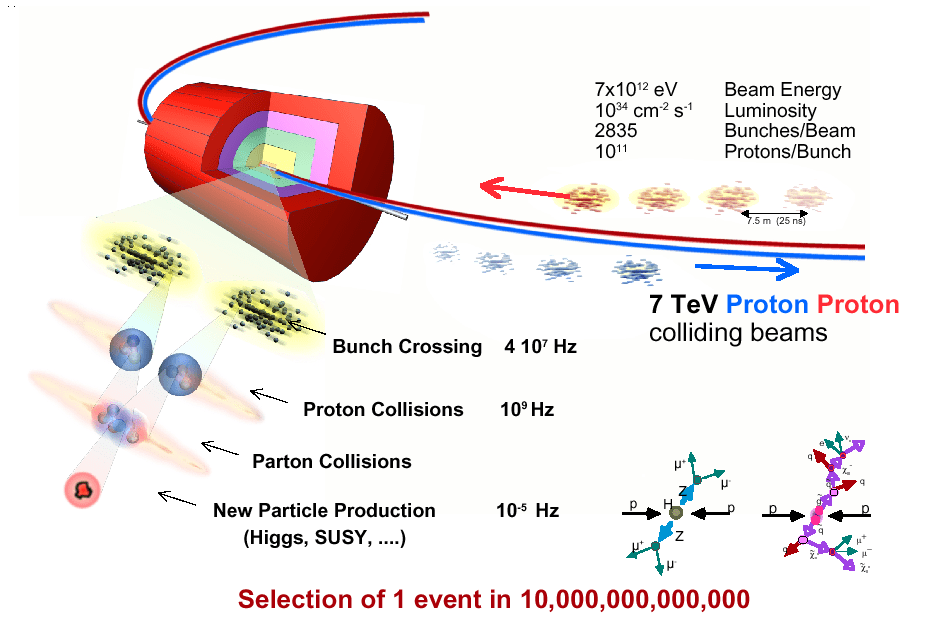
\includegraphics[width=.3\textwidth]{Imag/sketch_collisions.png}
%    \caption{Representac\'on de las colisiones en el Gran Colisionador de Hadrones}
\end{figure}
    
\end{frame}



\begin{frame}{Mas alla del modelo est\'andar. Modelo Dark-SUSY.}
Las nuevas fuerzas en el escenario Dark-SUSY puede asociarse al modelo est\'andar por medio de un termino de mezcla (kinetic mixing) que en forma de lagrangia tiene la siguiente forma: 

\begin{align*}
\mathcal{L}_{KM} &= - \frac{\epsilon}{2} F^{Y}_{\mu \nu} F^{D_{\mu \nu}} 
\end{align*} 

donde $F^{Y}_{\mu nu} = \partial_{\nu}A_{\nu}^{D} - \partial_{\nu}A_{\nu}^{D}$ es el campo de fuerzas en el sector oscuro. El rango tipico de $\epsilon$ es en el rango $10^{-8}$ - $10^{-2}$.
    
\end{frame}



\begin{frame}{Mas alla del modelo est\'andar. Modelo Dark-SUSY}
\begin{itemize}
\item Producci\'on de fotones oscuros por medio del portal del Higgs.
\item En este modelo el Higgs decae a particulas supersim\'etricas (neutralinos $n_{1}$)
\item subsequentemente cada neutralino decae a un neutralino oscuro ($n_{D}$) y un fot\'on oscuro ($\gamma_{D}$)
\item Cada fot\'on oscuro decae a un par de muones de carga opuesta\end{itemize}
\begin{figure}
\centering
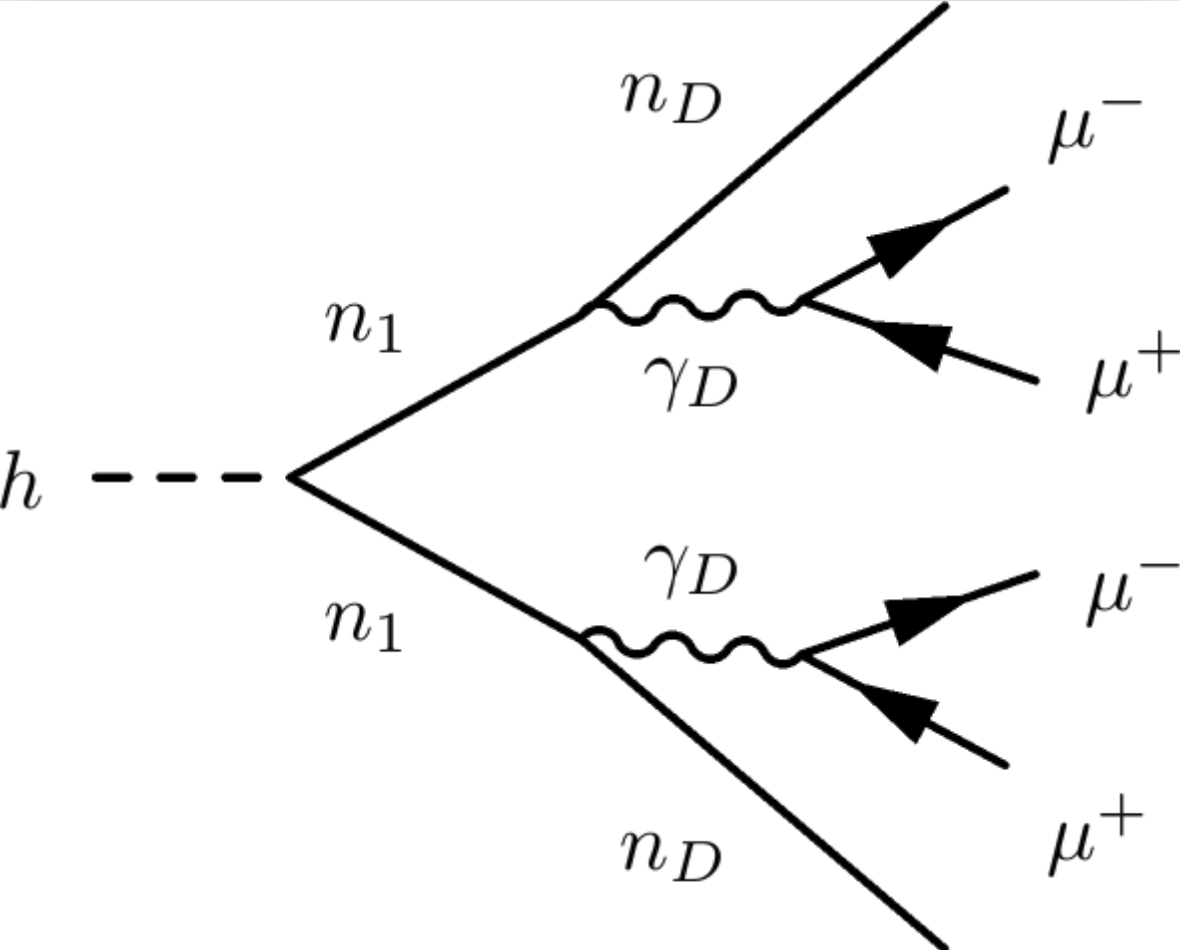
\includegraphics[width=.3\textwidth]{Imag/decae.png}
\caption{Diagrama de Feynman del modelo Dark-SUSY}
\end{figure}

\end{frame}

\begin{frame}{Mas alla del modelo est\'andar. Modelo Dark-SUSY}
Decaimiento del foton oscuro a leptones
\begin{itemize}
\item Debido al factor de mezcla $\epsilon$ el foton oscuro decae a leptones del modelo estandar con una anchura parcial dada por la siguiente expresion: 
\begin{equation}
\Gamma_{\gamma_{D}}\rightarrow \bar{l}l =\frac{1}{3}\alpha\epsilon^{2}m_{\gamma_{D}}\sqrt{1-\frac{4m_{l}^{2}}{m_{\gamma_{D}}^{2}}}\left(1+\frac{2m_{l}^{2}}{m_{\gamma_{D}}^{2}}\right)
\end{equation}

\end{itemize}
Donde $m_{l}$ es la masa del lepton (e,$\mu$, or $\tau$)    
\end{frame}


\begin{frame}{Mas alla del modelo est\'andar. Modelo Dark-SUSY}
Tiempo de vida\\
\begin{itemize}
\item El tiempo de vida esta relacionado a la anchura de decaimiento con la siguiente expresi\'on
\end{itemize}
\begin{equation}
\tau_{\gamma_{D}} = \frac{\hbar}{\Gamma_{\gamma_{D}}} \Rightarrow 
\tau_{\gamma_{D}}(\epsilon, m_{\gamma_{D}}) = \frac{1}{\epsilon^{2}}\times f(m_{\gamma_{D}})
\end{equation}
Es decir el tiempo de vida es una funci\'on de la masa del fot\'on oscuro y el par\'ametro de mezcla $\epsilon$. 

Es conveniente expresar el tiempo de vida como una distancia $c\tau_{\gamma_{D}}$, donde c es la velocidad de la luz. Tambi\'en es conveniente medir $c\tau_{\gamma_{D}}$ en milímetros para relacionar la sensitividad del modelo en el an\'alisis de datos. 
\begin{equation}
c\tau_{\gamma_{D}}(\epsilon,m_{\gamma_{D}})[mm] = \frac{c[mm/s]\times \hbar[GeV.s]}{\epsilon^{2}} \times f(m_{\gamma_{D}}[GeV^{-1}]
\end{equation}
\end{frame}


\begin{frame}{Propiedades del modelo}
\begin{figure}[ht]

\begin{minipage}[b]{0.45\linewidth}
\centering
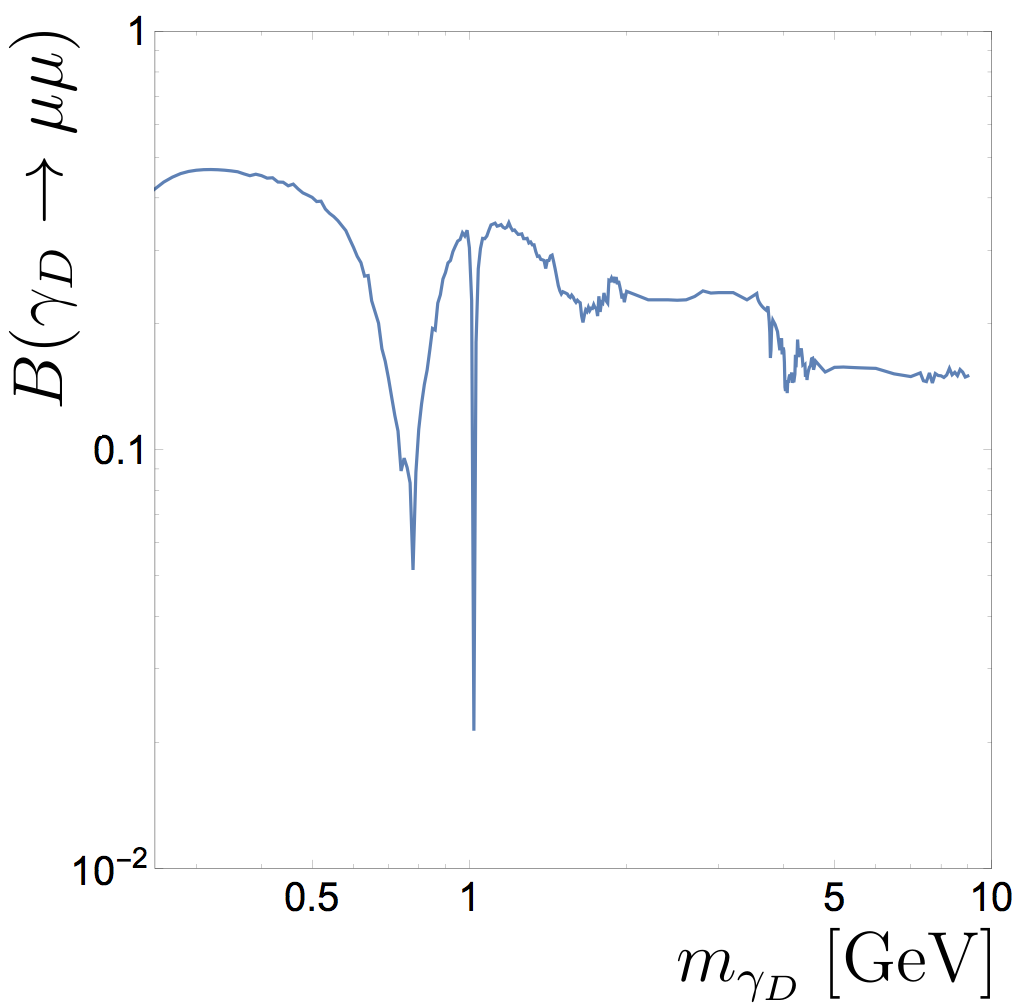
\includegraphics[width=1\textwidth]{Imag/teoria_dark_photon2.png}
\caption{Probabilidad de decaimiento del fotos oscuro a dos muones}
\end{minipage}
\hspace{0.5cm}
\begin{minipage}[b]{0.45\linewidth}
\centering
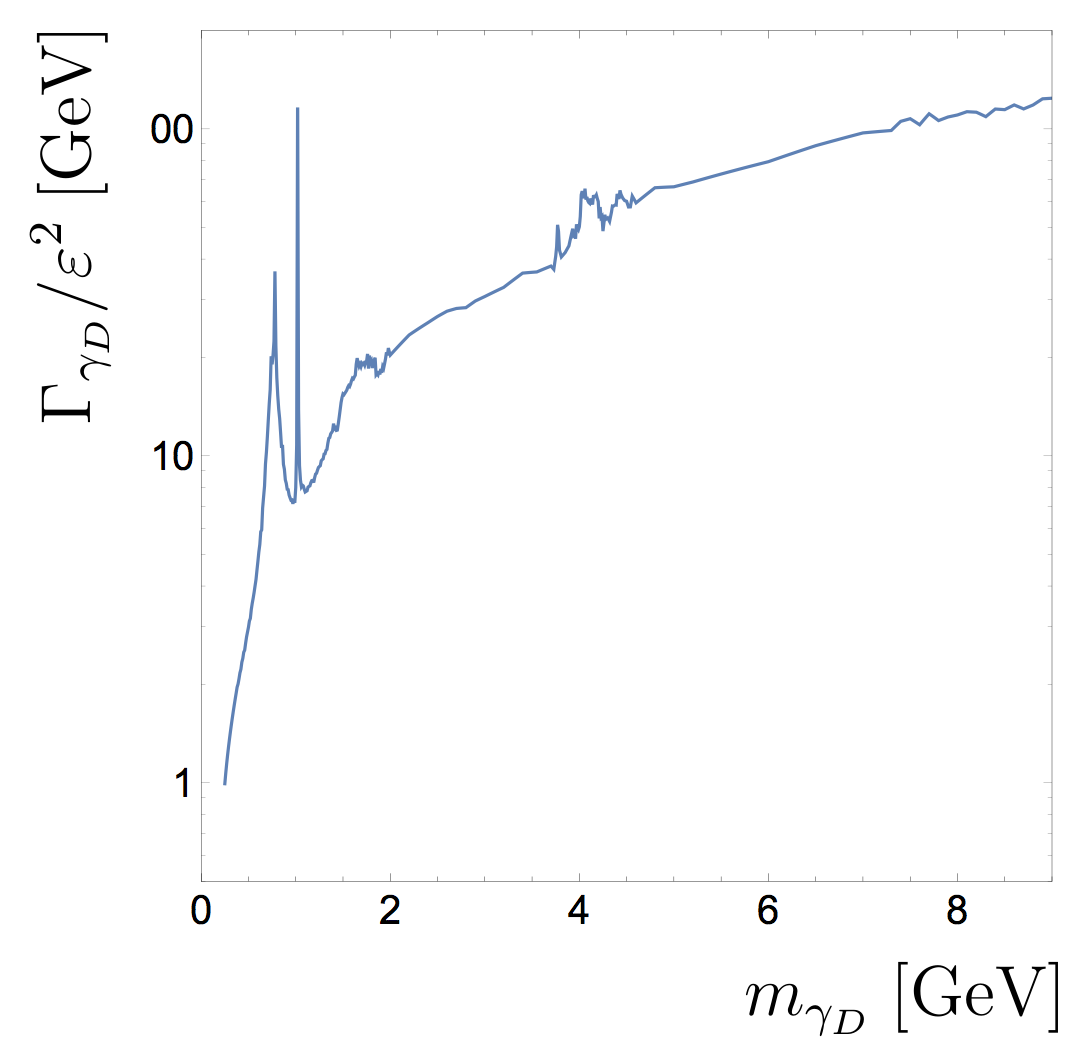
\includegraphics[width=1\textwidth]{Imag/teoria_dark_photon1.png}
\caption{Amplitud del decaimiento dividido por el coeficiente de mezcla cinetico}
\end{minipage}
\end{figure}
\end{frame}




% Teoría que intenta describir la existencia de materia oscura
% PROBLEMA, PROBLEMA, PROBLEMA, PROBLEMA, PROBLEMA
\begin{frame}{Problema de la investigaci\'on.}
%Dado que el modelo est\'andar no describe de forma \'exitosa como funciona el universo, part\'iculas hipot\'eticas derivadas de teor\'ias alternativas son necesarias para explicar estos fen\'omenos, y se hace necesario identificar la teoría desde limitaciones de los detectores.

Actualmente los modelos te\'oricos que predicen la formaci\'on de nuevas part\'iculas de materia oscura no han sido explorados ampliamente, por lo que no hay muchos m\'etodos desarrollados de identificaci\'on y caracterizaci\'on de las posibles se\~nales que ayuden a optimizar el proceso de calibraci\'on cuando se logre alcanzar el espacio fase de estos modelos.

\end{frame}


% HIPOTESIS, HIPOTESIS, HIPOTESIS, HIPOTESIS, HIPOTESIS
\begin{frame}{Hip\'otesis}
Si se hace supuesto que la materia oscura est\'a descrita por la teor\'ia MSSMD, al reconstruir la se\~nal desde los detectores por medio de la simulaci\'on es posible crear m\'etodos flexibles y eficientes de caracterizaci\'on, idenficaci\'on y reconstrucci\'on de las part\'iculas hipot\'eticas predichas por la teor\'ia.
\end{frame}


\begin{frame}{Objetivo General}
Estudiar por medio de simulaci\'on de Monte Carlo el modelo te\'orico ``Dark Susy'', reconstruyendo te\'oricamente las propiedades del fot\'on oscuro en un entorno simulado de los detectores que realizar\'ian la detecci\'on en configuraciones experimento CMS llamada Run-2 y en Alta Luminosidad.

\end{frame}


\begin{frame}{Objetivos espec\'ificos.}

\begin{itemize}
\item Recreaci\'on de la teor\'ia por medio de simulaci\'on mediante el desarrollo de un entorno de simulaci\'on y an\'alisis usando los recursos computacionales de la Universidad de Sonora (ACARUS).
%Estudio por medio de simulaci\'on de un modelo te\'orico que predice la creaci\'on de nuevas part\'iculas y fuerzas fundamentales.
%\item Dichas part\'iculas conocidas como fotones oscuros (Dark photons) son uno de los candidatos para explicar la composici\'on de la materia oscura en el universo.
\item Desarrollo de m\'etodos de identificaci\'on de la se\~nal a caracterizar.
\item Caracterizar la se\~nal en cuesti\'on y sus propiedades en el contexto del experimento CMS y sus futuras actualizaciones.
\end{itemize}
\end{frame}



\section{Simulaci�n}

\begin{frame}{}
    \begin{center}
        \LARGE Simulaci\'on
    \end{center}
\end{frame}


\begin{frame}{Simulaci\'on}

\begin{itemize}
    \item Para estudiar el modelo Dark-SUSY de forma experimental y caracterizar las propiedad de la se\~nal  
    se requiere generar muestras de simulaci\'on por el m\'etodo de Monte Carlo 
    \item La simulaci\'on requiere generar varias muestras considerando los par\'ametros m\'as importantes del fot\'on oscuro (masa y tiempo de vida) 
    \item Para generar las muestras simuladas se hace uso de paquetes propios del \'area de altas energ\'ias, los cuales act\'uan de forma sequencial y se encargan de diferentes aspectos del proceso de an\'alisis. 
\end{itemize}
    
\end{frame}


\begin{frame}{Paquetes de Simulaci\'on}
\begin{itemize}
    \item \textbf{Madgraph}: Se encarga de procesar la informaci\'on fundamental del modelo como la masa de las particulas madre, diagramas de Feynman, amplitudes de decaimiento, etc. 
    \item \textbf{Pythia}: Se encarga del proceso de hadronizaci\'on, es decir la interacci\'on entre protones, recombinaci\'on de quarks y formaci\'on de nuevas part\'iculas 
    \item \textbf{Delphes}: Se encarga de simular la respuesta del detector al paso de las part\'iculas simuladas, en este paso se consideran eficiencia de detecciones y se extraen variables como la energia, momento y trayectoria reconstruida de las part\'iculas en cuesti\'on
\end{itemize}

\end{frame}

\begin{frame}{Estrategia de Simulaci\'on}

\begin{itemize}
    \item Para generar las muestras se requiere crear un entorno automatizado (python) el cual pueda ser flexible a las diferentes variaciones del modelo
    \item Los archivos resultantes (formato .root) contienen la informaci\'on (teorica+experimental) para realizar el an\'alisis de datos.  
\end{itemize}

\begin{figure}[h]
\centering
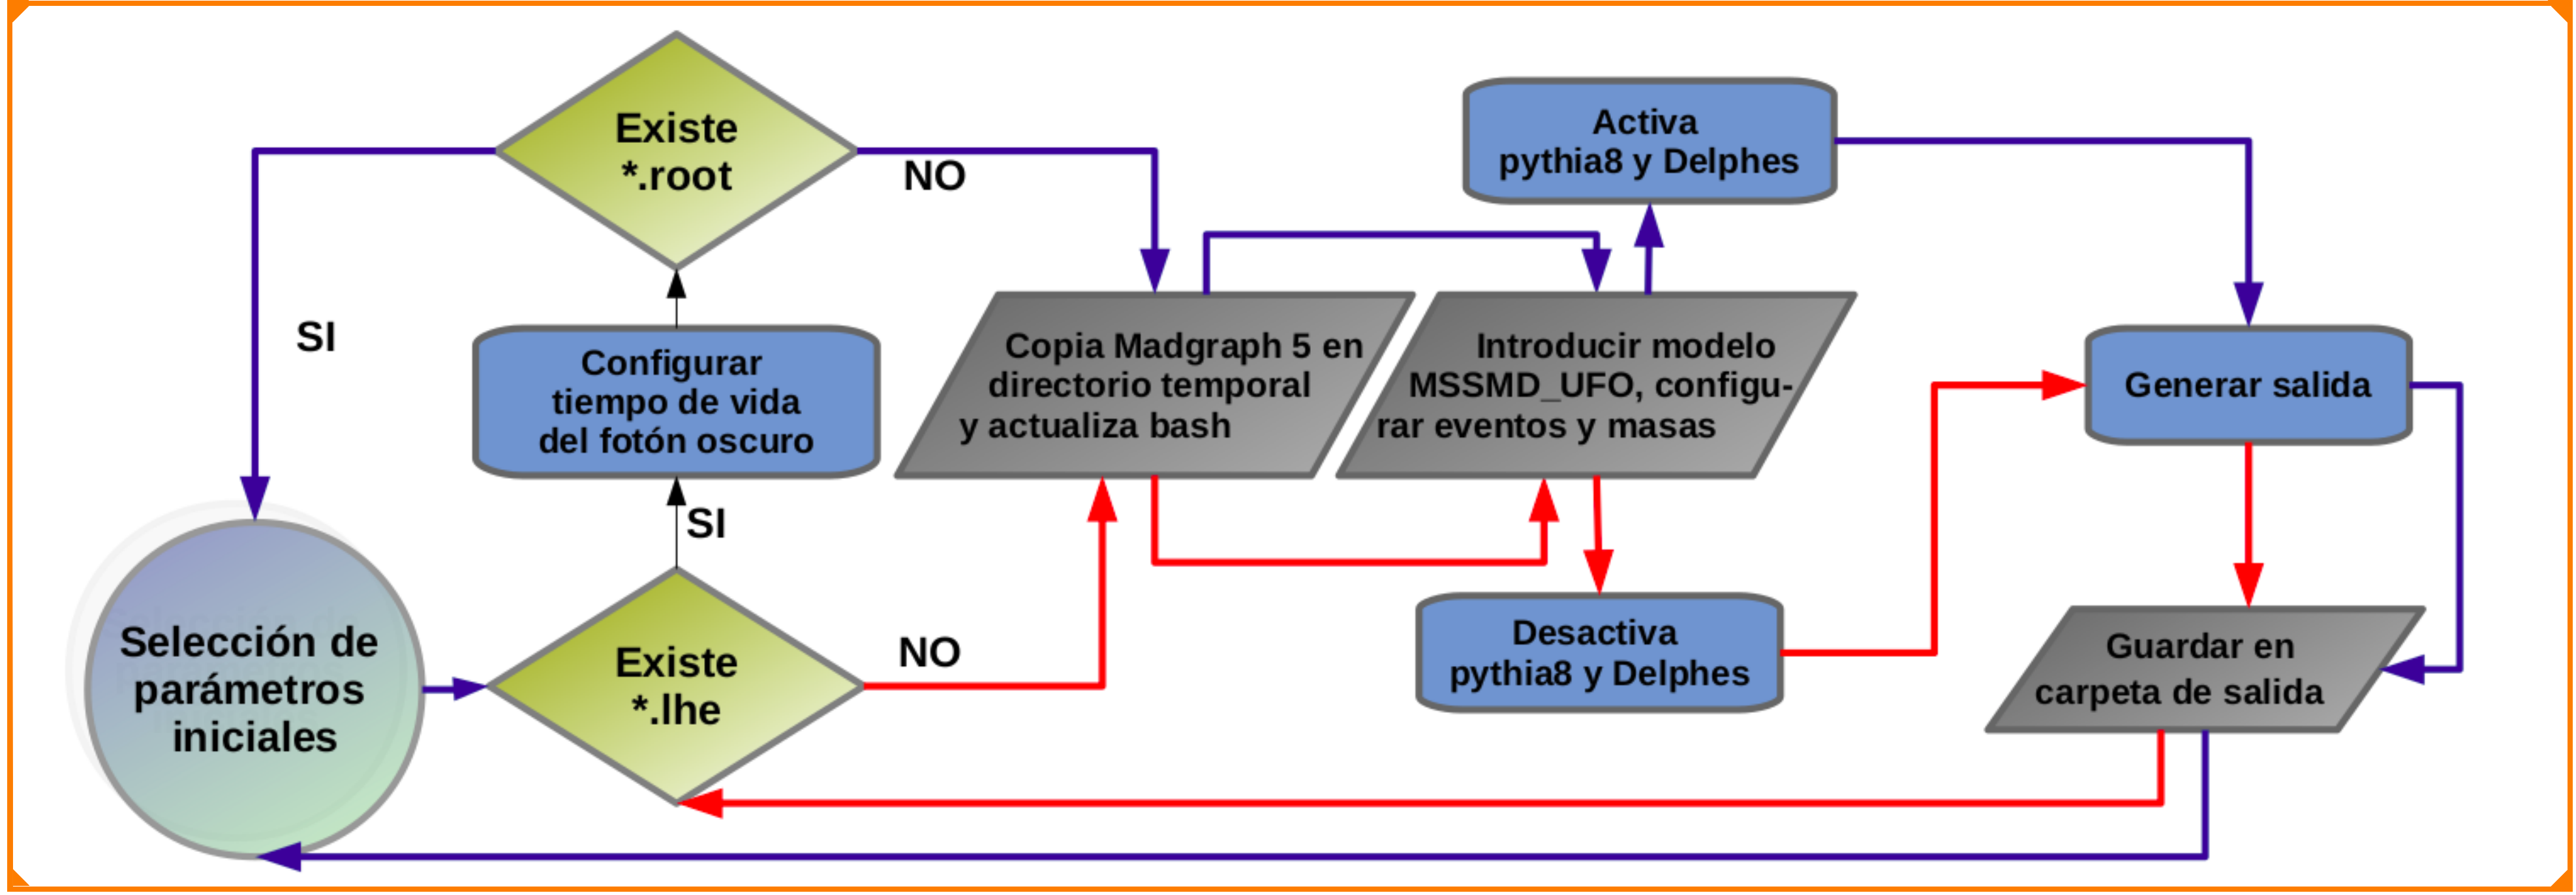
\includegraphics[width=0.8\textwidth]{Imag/proyecto_darksusy2.png}
\caption{Diagrama de Flujo del generador.}
\end{figure}

%Incluir diagrama donde se describa como se inicia la simulacion Madgraph->Pythia->Delphes
    
\end{frame}


\begin{frame}{Muestras simuladas}
    \begin{itemize}
        \item Para generar cada muestra se requiere especificar los siguientes par\'ametros: masa del neutralino ($m_{n_{1}}$), masa del dark neutralino ($m_{n_{D}}$), masa del fot\'on oscuro ($m_{\gamma_{D}}$) y tiempo de vida del foton oscuro ($c\tau_{\gamma_{D}}$) que son los par\'ametros del modelo Dark-SUSY. 
        %\item El numero de muestras simuladas se representa en la siguiente tabla
        \item El n\'umero de muestras simuladas es el resultado de todas las combinaciones posibles de los vectores correspondientes a los par\'ametros de generaci\'on, haciendo un total de $\backsim 15 000$ muestras:
    \end{itemize}

\begin{table}
\begin{footnotesize}
\begin{tabular}{|cl|}
\hline
$V_{m_{n_{1}}}$ & = $[10, ~20, ~30, ~40, ~50, ~60, ~70, ~80, ~90, ~100]$\\
$V_{m_{n_{D}}}$ & = $[0.25, ~1, ~2, ~3, ~4, ~5, ~10]$\\
$V_{m_{\gamma_{D}}}$ & = $[0.25, ~1, ~2, ~3, ~4, ~5, ~6, ~7, ~8, ~9, ~10]$\\
$V_{c\tau_{\gamma_{D}}}$ & = $[0, ~1, ~2, ~3, ~4, ~5, ~10, ~20, ~30, ~40, ~50, ~100]$\\
Eventos simulados &  = 10000\\
\hline
\hline
\end{tabular}
\end{footnotesize}
\end{table}
\end{frame}




%\begin{comment}

%\begin{frame}{Muestras simuladas}
%Notaci\'on:\\
%$\mathbb{E}_i^{(j,~k)} ~= ~1$  hace referencia a los eventos, donde $i = \{1, \ldots, i_{max}\}$ corresponde al elemento del evento en el \'arbol de archivo $*.root$ requerido, y donde: $\{j, ~k\} = \{\{0\mu, ~1\mu, ~2\mu, ~3\mu, ~4\mu\, \ldots\},\{\mathtt{CMS},~\mathtt{HL}\}\}$ hace referencia a los eventos seg\'un su contenido mu\'onico y al detector que gener\'o los datos. Entonces:
%\begin{equation*}
%\mathbb{E}^{(j,~\mathtt{CMS})} = \sum_i \mathbb{E}_i^{(j, ~\mathtt{CMS})} , ~~~~ \mathbb{E}_i^{(\mathtt{CMS})} = \sum_j \mathbb{E}_i^{(j,~\mathtt{CMS})} ~~~~ y ~~~~ \mathbb{E}^{\mathtt{(CMS)}}= \sum_{ij} \mathbb{E}_i^{(j,~\mathtt{CMS})}
%\end{equation*}
%\begin{equation*}
%\mathbb{E}^{(j,~\mathtt{HL})} = \sum_i \mathbb{E}_i^{(j, ~\mathtt{HL})} , ~~~~ \mathbb{E}_i^{(\mathtt{HL})} = \sum_j \mathbb{E}_i^{(j,~\mathtt{HL})} ~~~~ y ~~~~ \mathbb{E}^{\mathtt{(HL)}}= \sum_{ij} \mathbb{E}_i^{(j,~\mathtt{HL})}
%\end{equation*}
%donde:
%\begin{equation*}
%\mathbb{E}^{(j,~k)}\equiv \mathbb{E}^{(j,~k)}\mathtt{(MNeuL,~MNeuD,~MPhoD,~TcPhoD)}
%\end{equation*}
%
%\end{frame}



%\begin{frame}{Muestras simuladas}
%Notaci\'on:\\
%\begin{equation*}
%f^{(j,~k)} = \dfrac{\mathbb{E}^{(j,~k)}}{\mathbb{E}^{(k)}}
%\end{equation*}
%Para el caso que nos ocupa $\mathbb{E}^{(k)} ~= ~\mathtt{Event} ~= ~10 000$ son los eventos simulados para cada configuraci\'on requerida. Ejemplos:
%\begin{table}
%\begin{footnotesize}
%\begin{tabular}{|cccccc|}
%\hline
%$\texttt{MNeuL(GeV)}$ & $\texttt{MNeuD(GeV)}$ & $\texttt{MPhoD(GeV)}$ & $\texttt{TcPhoD(mm)}$ & $f^{(4\mu,~\texttt{CMS})}$ & $f^{(4\mu,~\texttt{HL})}$ \\
%\hline
%10 & 0.25 & 0.25 & 0.5 & 0.0920 & 0.1678\\
%& & & 2 & 0.0779 & 0.1355 \\
%& & & 4 & 0.0597 & 0.1024 \\
%& & & 10 & 0.0227 & 0.0433 \\
%& & & 50 & 0.0016 & 0.0039 \\
%\hline
%10 & 0.25 & 0.25 & 2 & 0.0497 & 0.1135 \\
%& & 4 & & 0.0494 & 0.1157 \\
%& & 6 & & 0.0599 & 0.1456 \\
%& & 8 & & 0.0957 & 0.1960 \\
%\hline
%\end{tabular}
%\end{footnotesize}
%\end{table}

%\begin{table}[]
%    \centering
%    \begin{tabular}{c|c|c|}  \hline
%    Masa [GeV]     & Tiempo de vida [mm]  &  Numero de eventos \\ \hline 
%         &  & \\ \hline 
%         & & \\ \hline 
%    \end{tabular}
%    \caption{Muestras simuladas del modelo Dark-SUSY}
%    \label{tab:my_label}
%\end{table}  
%\end{frame}
%\end{comment}


\begin{frame}{Simulaci\'on del Detector en Delphes}

\begin{itemize}
    \item Delphes es un paquete de simulaci\'on rapida, es decir alguna de las eficiencias de deteccion estan parametrizadas, lo anterior para reducir el tiempo de simulaci\'on 
    \item Dichar parametrizaciones se obtienen de la simulaci\'on mas detallada (Geant4) la cual contempla todos los procesos fundamentales del paso de las particulas por el detector
    \item En nuestro modelo los fotones oscuros decaen a muones, por lo que la reconstrucci\'on de los mismos es parte fundamental del an\'alisis
\end{itemize}
\end{frame}


\begin{frame}{Identificaci\'on de muones en CMS}
    
\begin{itemize}
\item Los muones son particulas elementales que interaccionan d\'ebilmente con la materia, su trayectoria se reconstruye con informaci\'on obtenida de detectores dedicados a esta tarea
\item A partir de la trayectoria reconstruida y la desviaci\'on provocada por el campo magn\'etico solenoide se puede obtener el valor del momento.
\item Debido a que el fot\'on oscuro puede viajar una distancia considerable antes de decaer la eficiencia de reconstrucci\'on de muones esta \'intimamente ligado al tiempo de vida (c$\tau$) 
\item En general se espera que a mayor tiempo de vida del fot\'on oscuro la eficiencia de identificaci\'on es menor (debido a que los muones logran atravesar solo una parte de los dispositivos de detecci\'on)
\end{itemize}
\end{frame}


\begin{frame}{Identificaci\'on de muones en CMS}

\begin{itemize}
    \item La linea azul representa el paso de los muones por el detector CMS
\end{itemize}

\begin{figure}
    \centering
    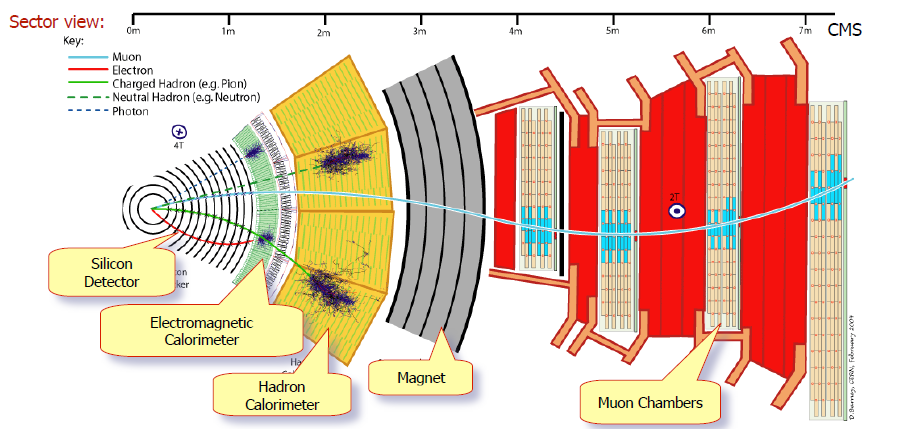
\includegraphics[width=0.8\textwidth]{Imag/reconstruccion_muones.png}
    \caption{Identificaci\'on de part\'iculas en CMS, vista transversal del detector}
    \label{fig:my_label}
\end{figure}
    
\end{frame}



\begin{frame}{Definici\'on de variables relevantes}
El detector CMS tiene una simetr\'ia cilindrica en donde el eje de colisi\'on es el ``z'' y el plano transversal esta formado por los ejes ``x'' e ``y''. Dos de las variables para caracterizar las propiedades de las part\'iculas son las siguientes. 
\begin{figure}[ht]
\begin{minipage}[b]{0.45\linewidth}
\centering
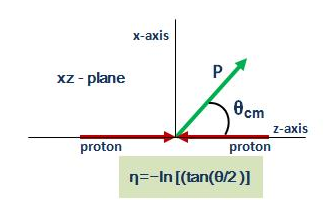
\includegraphics[width=\textwidth]{Imag/pseudorapidity.PNG}
\caption{Definici\'on de pseudorapidez}
\end{minipage}
\hspace{0.5cm}
\begin{minipage}[b]{0.45\linewidth}
\centering
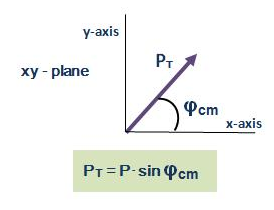
\includegraphics[width=\textwidth]{Imag/pt.PNG}
\caption{Definici\'on de momento transversal}
\end{minipage}
\end{figure} 

\end{frame}



\begin{frame}{Parametrizaci\'on de eficiencia y resoluci\'on}

Estas parametrizaci\'on est\'an contenidas en la simulaci\'on Delphes
\begin{figure}[ht]
\begin{minipage}[b]{0.45\linewidth}
\centering
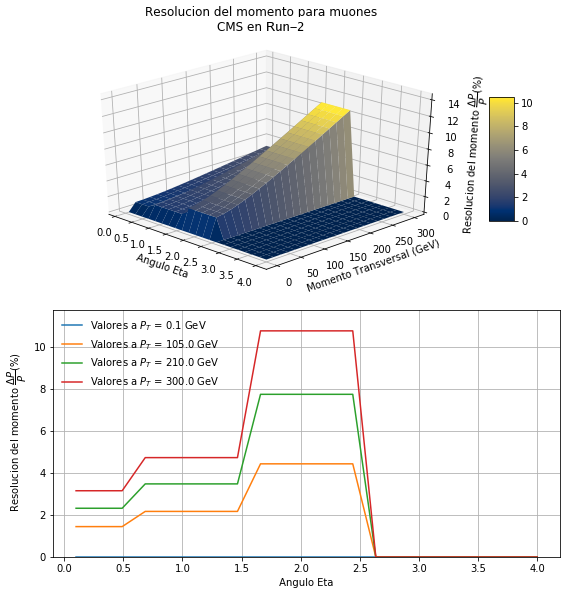
\includegraphics[width=\textwidth]{Imag/Momentum_resolution_of_Muon_CMS.png}
\caption{Resoluci\'on del momento para muones.}
\end{minipage}
\hspace{0.5cm}
\begin{minipage}[b]{0.45\linewidth}
\centering
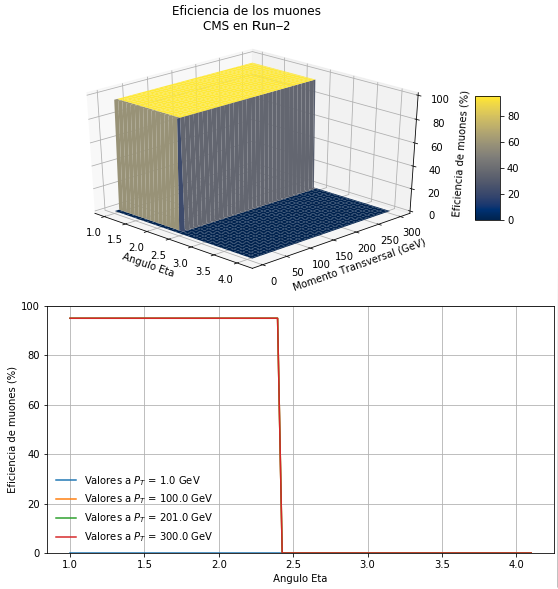
\includegraphics[width=\textwidth]{Imag/Eficiencia_of_Muon_CMS.png}
\caption{Eficiencia en la reconstrucci\'on de los muones.}
\end{minipage}
\end{figure}
    
\end{frame}

\section{An\'alisis}

\begin{frame}{}
    \begin{center}
        \LARGE An\'alisis
    \end{center}
\end{frame}


\begin{frame}{Estrategia del an\'alisis de datos}
\begin{itemize}
\item El an\'alisis se basa en una selecci\'on de eventos a partir de una serie de variables experimentales las cuales buscan optimizar la eficiencia de la se\~nal y reducir lo mas posible los procesos de ruido.
\item Recordar que en los datos experimentales solo se tiene informaci\'on de los muones reconstruidos y a partir de eso se infiere la posible producci\'on de fotones oscuros.
\item La selecci\'on de eventos se aplica a cada una de las muestras de simulaci\'on generadas y se estudia las eficiencias y distribuciones caracter\'isticas.
\end{itemize}    
\end{frame}


\begin{frame}{Secuencia del an\'alisis de datos}

\begin{itemize}
    \item El an\'alisis comienza con la muestra simulada (raw data) 
    \item Se procede a la selecci\'on de eventos, donde se reduce la cantidad de datos a analizar 
    \item Se procede a la obtenci\'on de resultados, gracias estad\'isticas y discusi\'on de los mismos, algo similar al esquema mostrado en la figura 
\end{itemize}


\begin{figure}[h]
\centering
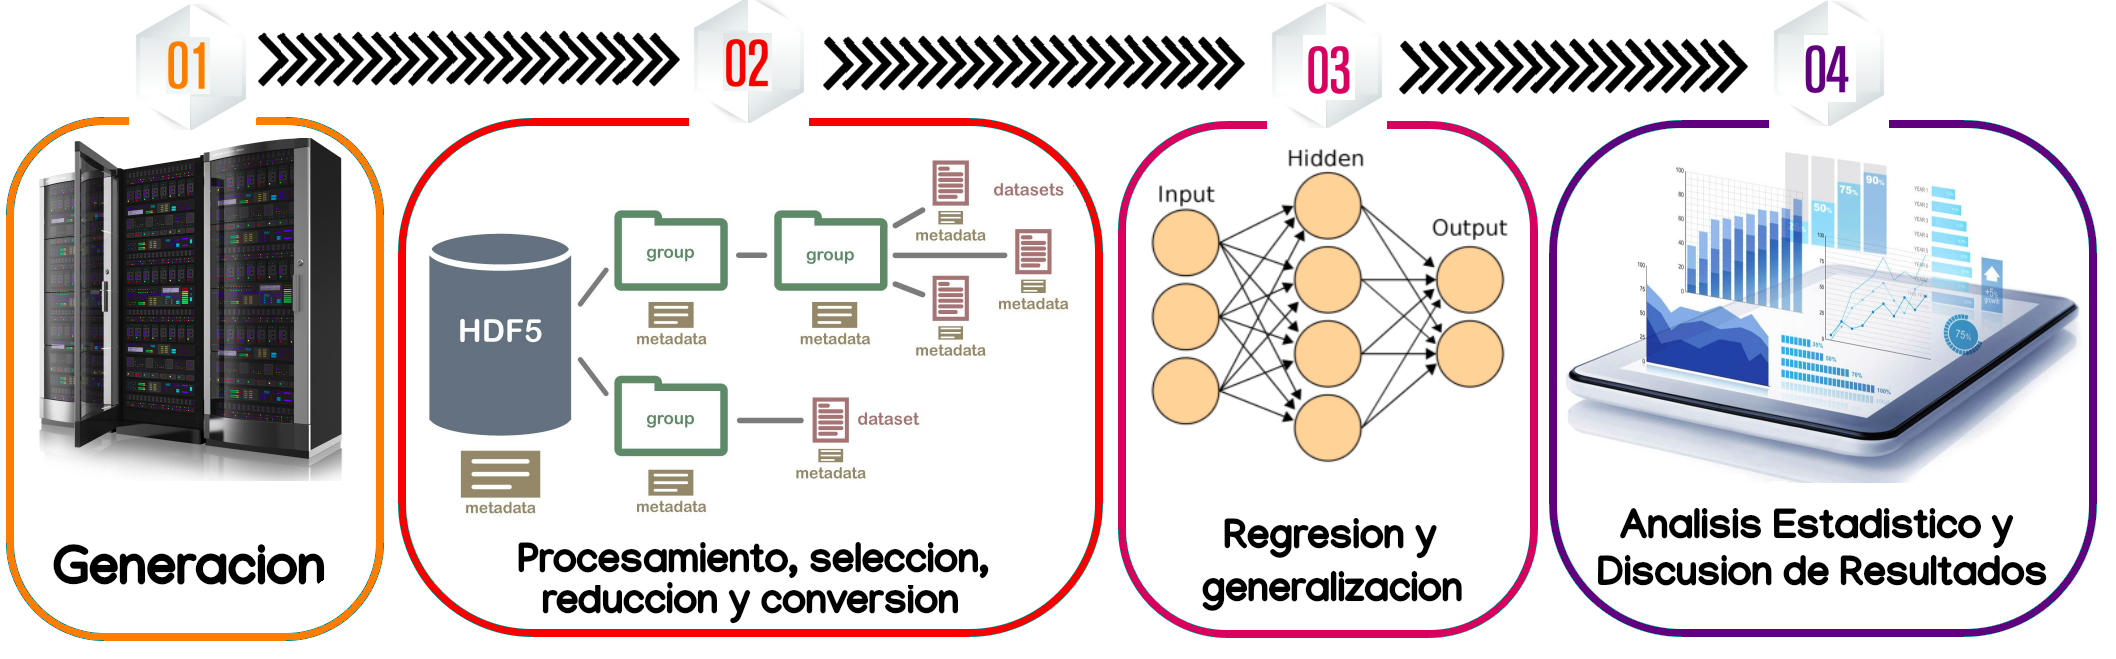
\includegraphics[width=0.8\textwidth]{Imag/procesos_darksusy.png}
\caption{Secuencia del an\'alisis de datos}
\end{figure}

\end{frame}


\begin{frame}{Estructura del c\'odigo de an\'alisis}

\begin{itemize}
    \item Se desarrollo un entorno de simulaci\'on y an\'alisis de datos el cual esta basado en c\'odigo de python y ROOT. 
    \item El entorno se encuentra hospedado en ACARUS y puede ser f\'acilmente extendido para el an\'alisis de otros modelos (adicionales a Dark-SUSY)
\end{itemize}
    
\begin{figure}[h]
\centering
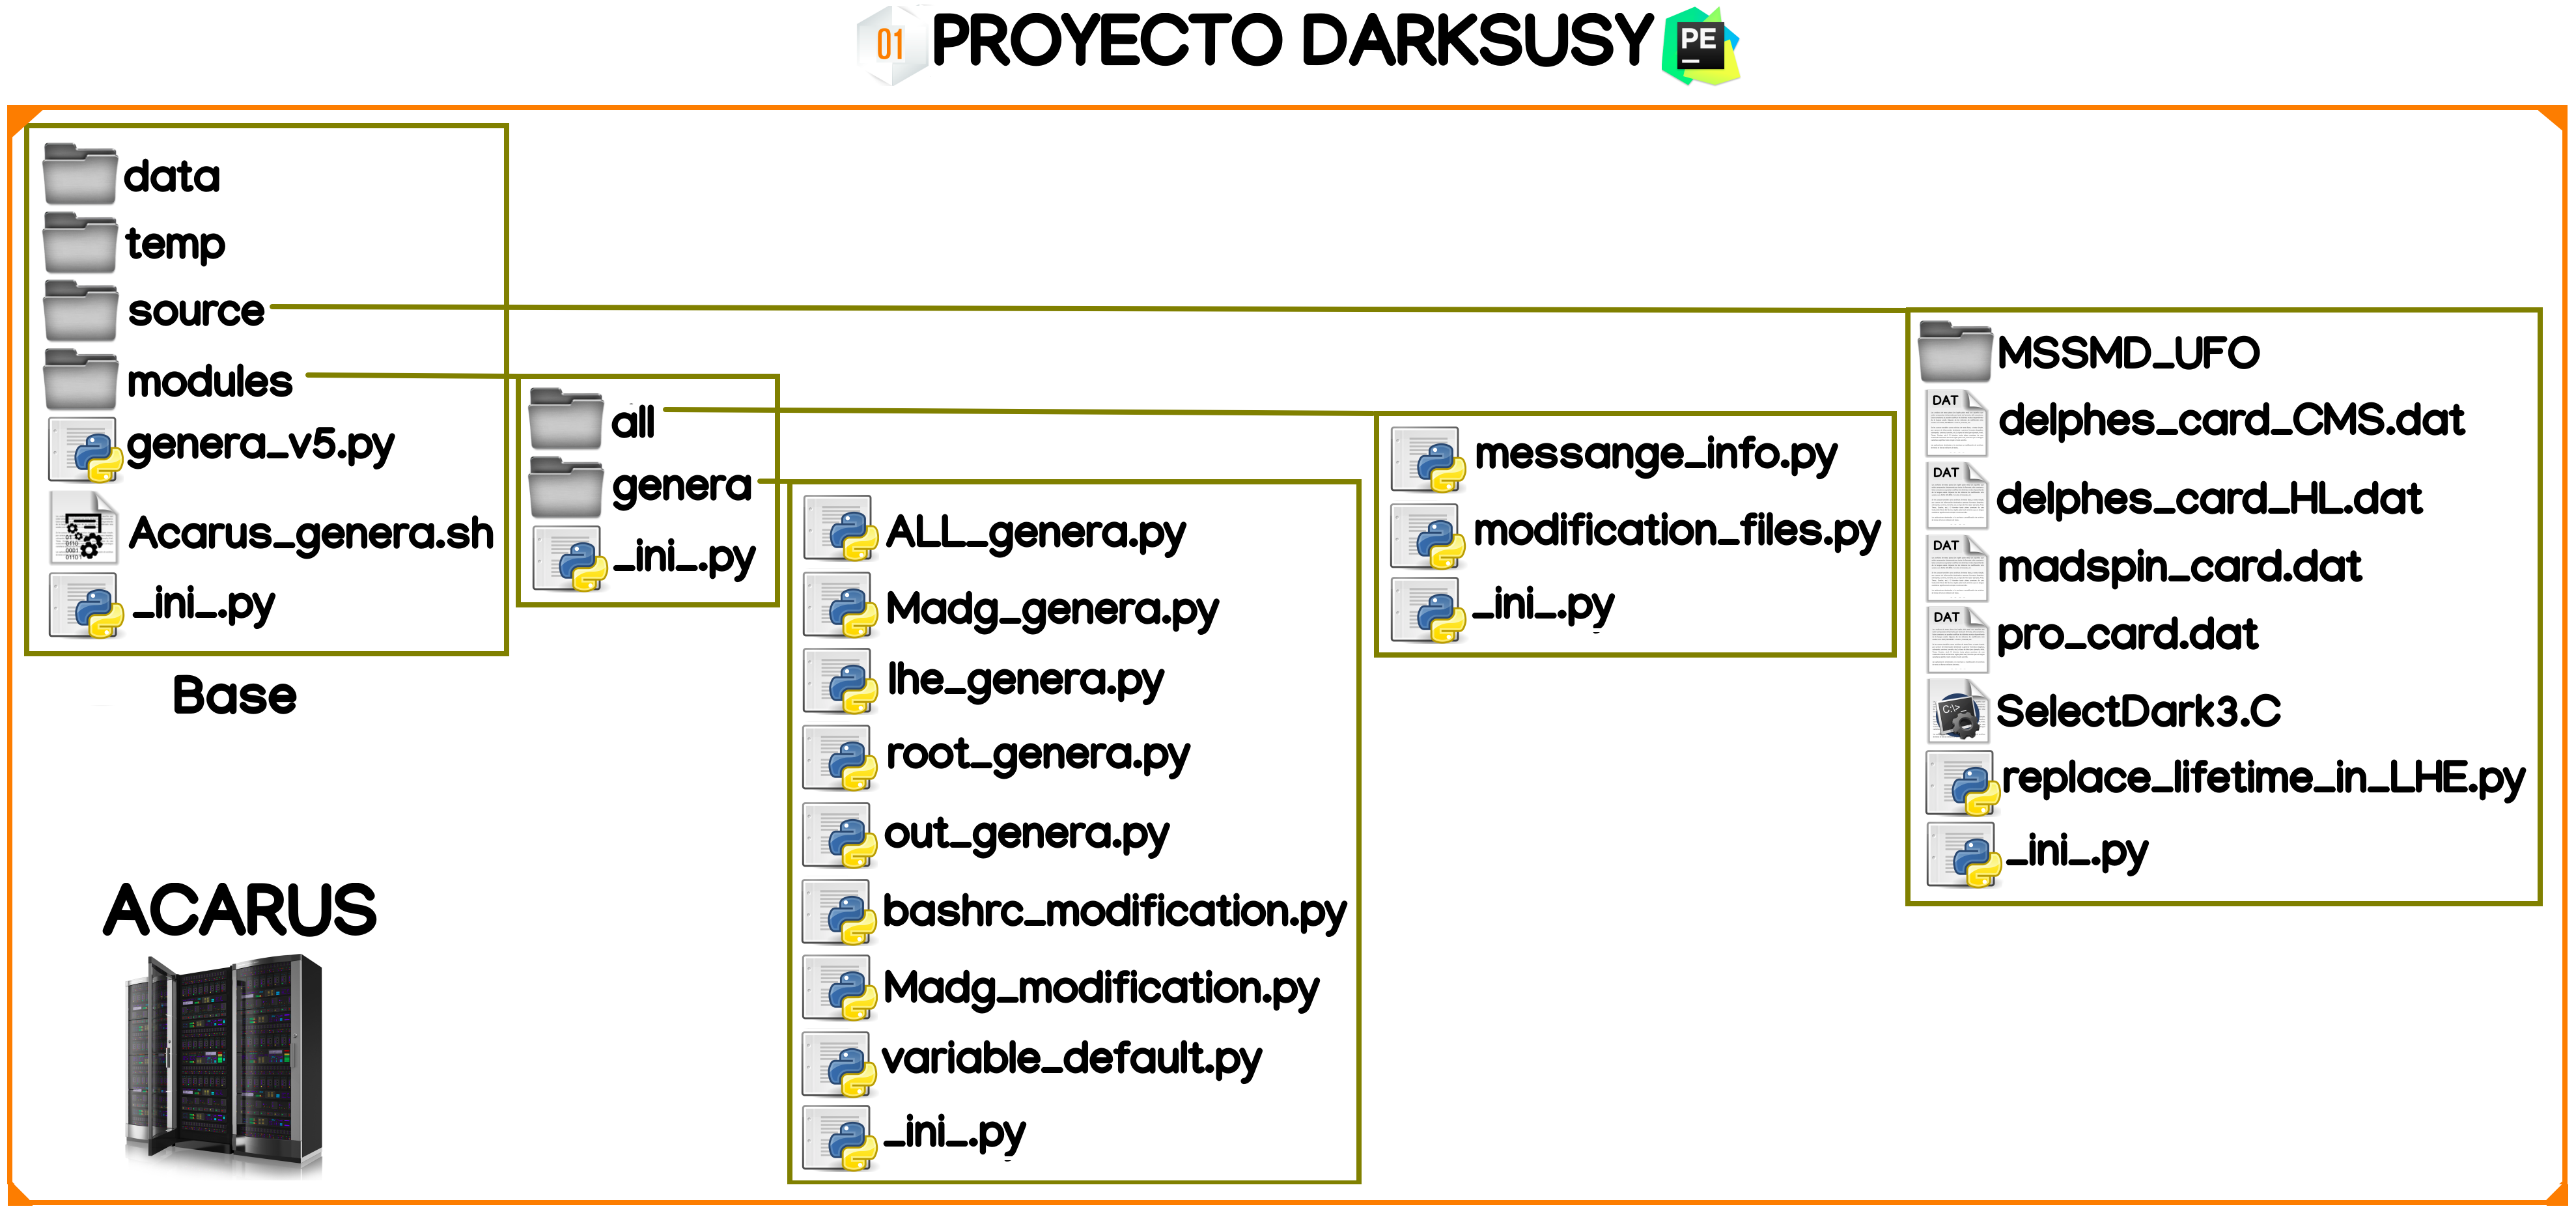
\includegraphics[width=0.8\textwidth]{Imag/proyecto_darksusy.png}
\caption{Estructura del c\'odigo de an\'alisis}
\end{figure}

\end{frame}



\begin{frame}{Selecci\'on preliminar}

\begin{itemize}
%\item \textbf{4$\mu$}: Selecci\'on de eventos con al menos 4 muones
%	\begin{itemize}
%		\item Muones con un momento transversal ($p_{T}$) mayor a
%		\item Muones con un valor de pseudo-rapidez ($|\eta|$) menor a 2.4
%	\end{itemize}
\item \textbf{Algoritmo de pariamiento de muones}: Encontrar el par de muones \'optimos que con mayor probabilidad podr\'ian ser generados por un fot\'on oscuro.

\item \textbf{Algoritmo con identificador de machine learning di-muon}: Optimizas la detecci\'on haciendo conocida las muestras y pareamientos reales con la paqueter\'ia de tensorflow.

\end{itemize}
    
\end{frame}


\begin{frame}{Algoritmo de pariamiento de muones}
% \color{red} Francisco aqui incluir el diagrama de algoritmo de pariamiento
\begin{figure}[h]
\centering
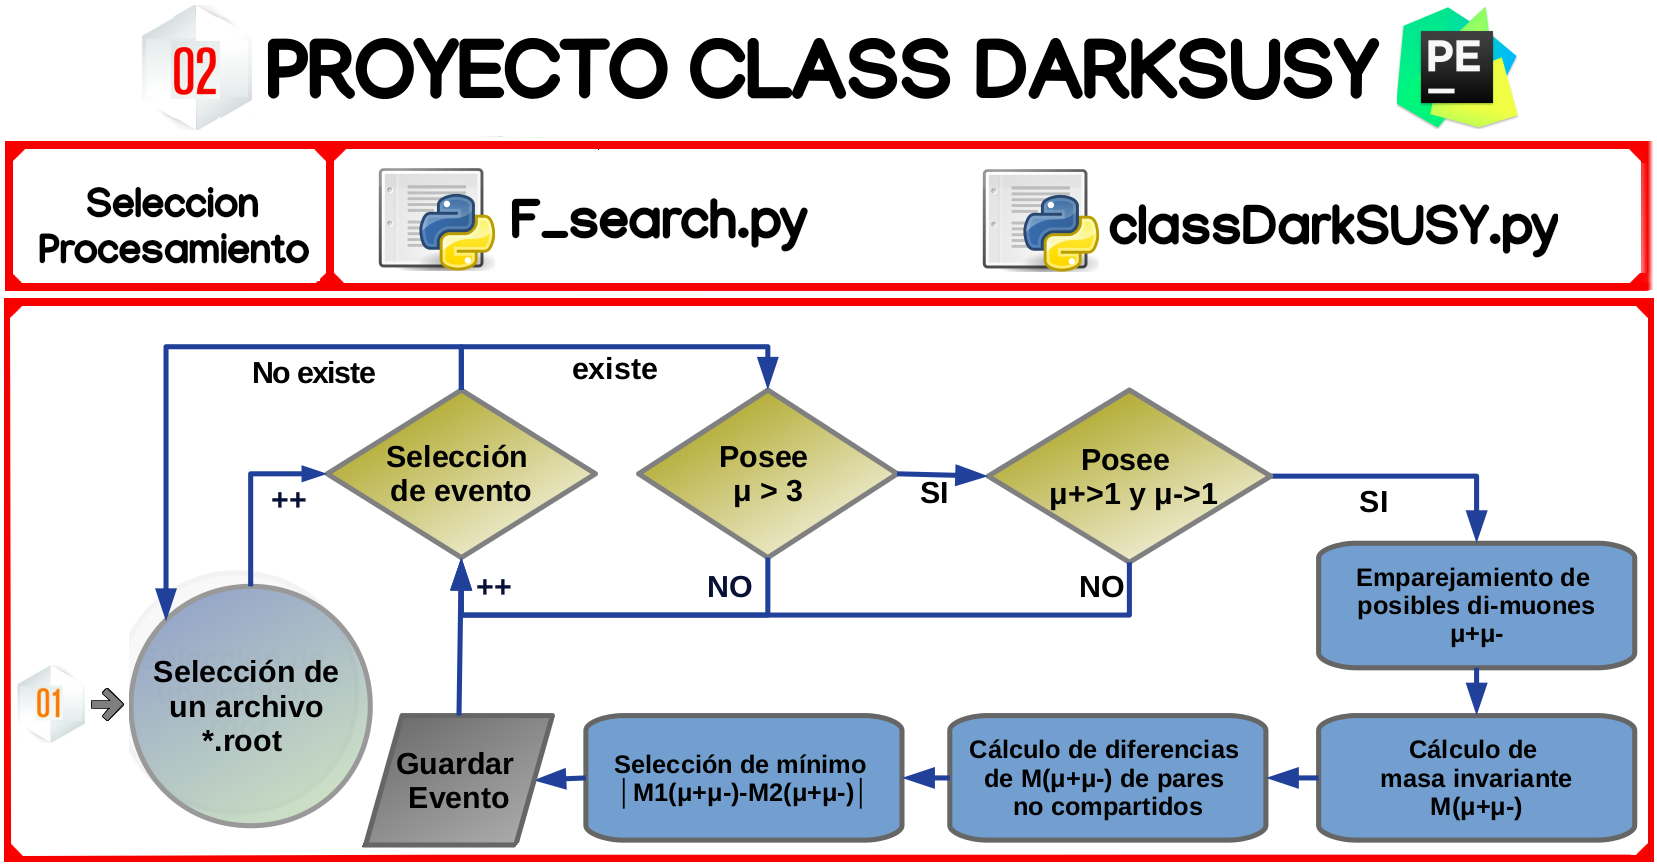
\includegraphics[width=1\textwidth]{Imag/class_darksusy.png}
\caption{Diagrama de algoritmo de pariamiento. Eficiencia conocida de 87\%.}
\end{figure}   
\end{frame}


\begin{frame}{Algoritmo con identificador de machine learning di-muon}
Proceso de entrenamiento y creaci\'on del modelo.
\begin{figure}[h]
\centering
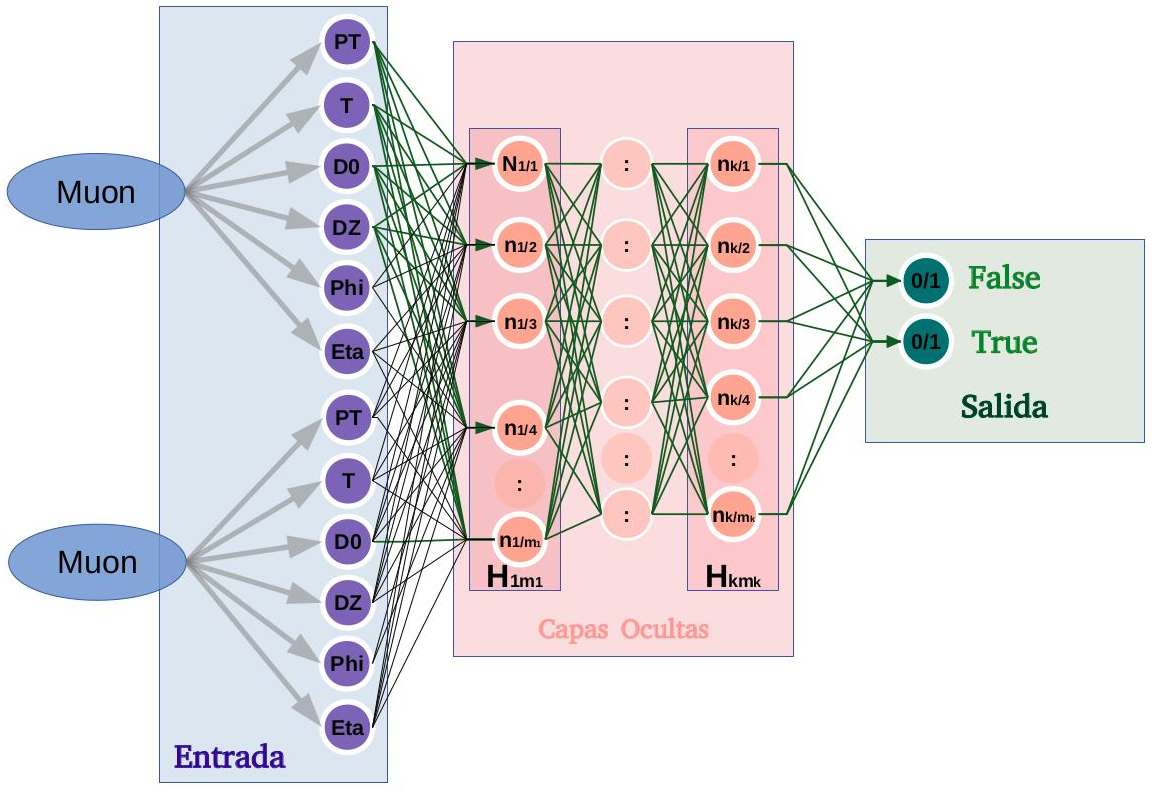
\includegraphics[width=.8\textwidth]{Imag/IDENTIFICADOR.png}
\caption{Creaci\'on del identificador. Eficiencia conocida de 98\%.}
\end{figure}   
\end{frame}


\begin{frame}{Eficiencia para fot\'on oscuro con detector CMS}
\begin{small}
%\color{red} Francisco llenar estos numeros \color{black}
\begin{table}[]
\centering
\begin{tabular}{c|c|c|c|c|c|}
Selecci\'on  & $c\tau=0.5$ & $c\tau=5$ & $c\tau=10$ & $c\tau=50$ & $c\tau=100$ \\  \hline
Sin corte    &  10 000 & 10 000 & 10 000 & 10 000 & 10 000\\
4-$\mu$      &  916 & 500 & 227 & 16 & 2 \\
pariamiento  &  916 & 500 & 227 & 16 & 2
\end{tabular}
\caption{Tabla con el numero de eventos despu\'es de cada selecci\'on $m_{\gamma_{D}}$=0.25 GeV y diferentes valores del tiempo de vida para el detector CMS.}
\end{table}

\begin{table}[h]
\centering
\begin{tabular}{c|c|c|c|c|c|}
Selecci\'on  & $c\tau=0.5$ & $c\tau=5$ & $c\tau=10$ & $c\tau=50$ & $c\tau=100$ \\ \hline
Sin corte   & 10 000 & 10 000 & 10 000 & 10 000 & 10 000\\
4-$\mu$     & 955 & 968 & 947 & 862 & 655 \\
pariamiento & 955 & 968 & 947 & 862 & 655
\end{tabular}
\caption{Tabla con el n\'umero de eventos despu\'es de cada selecci\'on $m_{\gamma_{D}}~=~ 8~GeV$ y diferentes valores del tiempo de vida para el detector CMS.}
\end{table}

\end{small}

\end{frame}



\begin{frame}{Distribuciones caracter\'isticas: Masa invariante}
    
\begin{itemize}
\item Despu\'es de la selecci\'on preliminar se puede reconstruir la masa de los muones, dicha masa corresponder\'ia a la masa de los fotones oscuros. A continuaci\'on se muestra un ejemplo para los procesos con un valor esperado de $m_\gamma = 4 GeV$: 
\end{itemize}
    
\begin{figure}[ht]
\centering
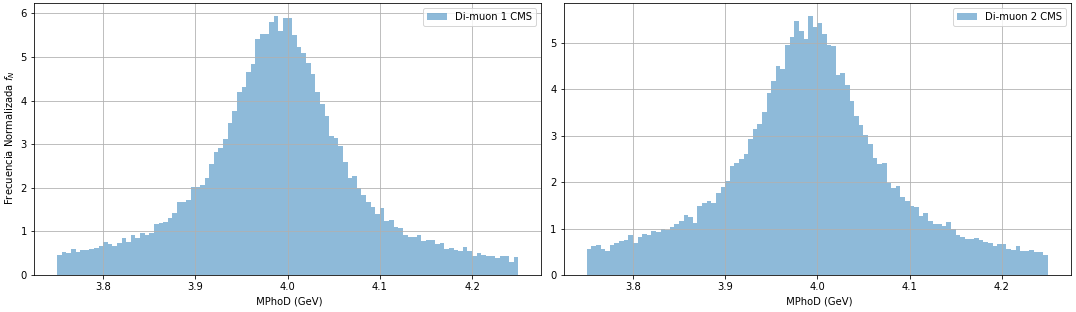
\includegraphics[width=1\textwidth]{Imag/Datos_Photon4muon_CORTE_CMS.png}
\caption{Masa invariante para los di-muones.}
\end{figure}
%\begin{figure}[ht]
%\begin{minipage}[b]{0.45\linewidth}
%\centering
%
\includegraphics[width=1\textwidth]{Imag/placeholder.png}
%\caption{Masa invariante primer di-muon}
%\end{minipage}
%\hspace{0.5cm}
%\begin{minipage}[b]{0.45\linewidth}
%\centering
%
\includegraphics[width=1\textwidth]{Imag/placeholder.png}
%\caption{Masa invariantes segundo di-muon}
%\end{minipage}
%\end{figure}
\end{frame}



\begin{frame}{Distribuciones caracter\'isticas: Par\'ametros}

\begin{figure}[h]
\centering
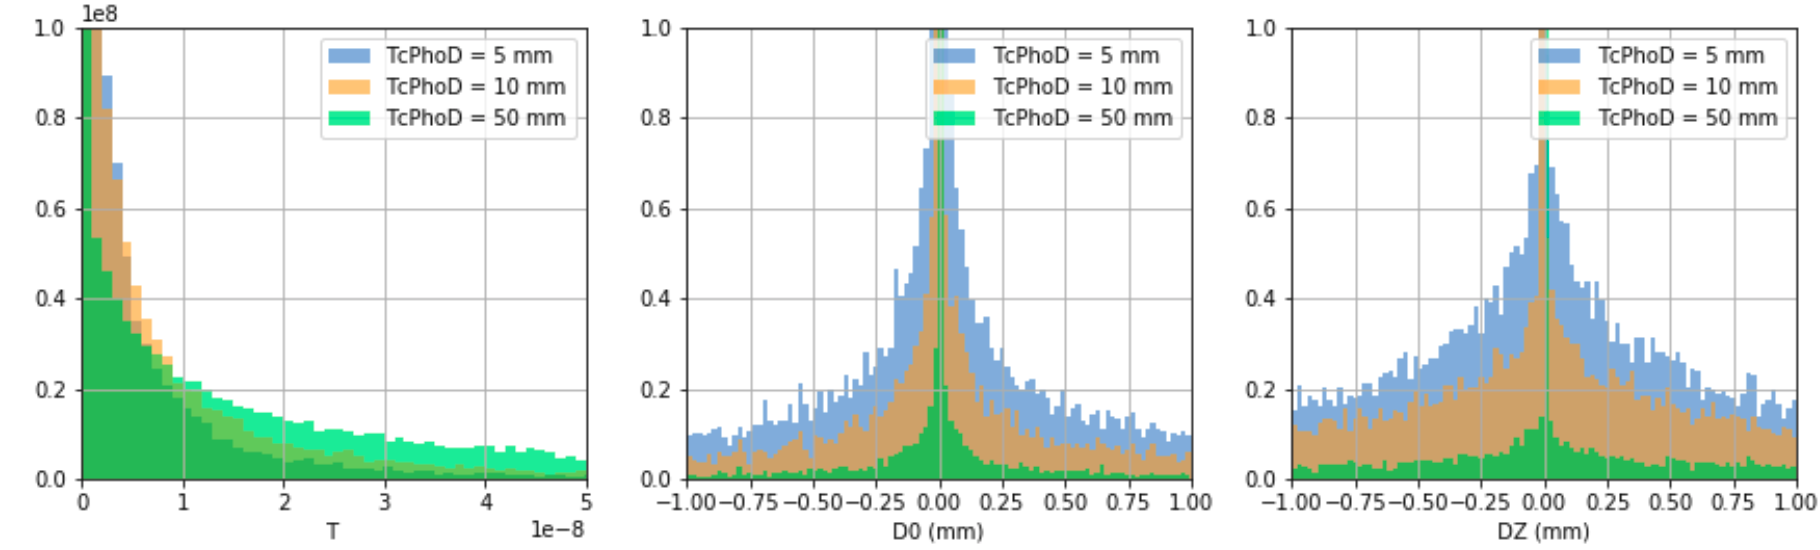
\includegraphics[width=1\textwidth]{Imag/variar_parametros.png}
\caption{Variaciones de algunas propiedades del muon con el cambio de tiempo de vida del f\'oton oscuro.}
\end{figure} 

\end{frame}


\begin{frame}{}
    \begin{center}
        \LARGE High Luminosity LHC
    \end{center}
\end{frame}


\begin{frame}{Eficiencia para fot\'on oscuro para detector HL.}
\begin{small}
%\color{red} Francisco llenar estos numeros \color{black}
\begin{table}[]
\centering
\begin{tabular}{c|c|c|c|c|c|}
Selecci\'on  & $c\tau=0.5$ & $c\tau=5$ & $c\tau=10$ & $c\tau=50$ & $c\tau=100$ \\  \hline
Sin corte    &  10 000 & 10 000 & 10 000 & 10 000 & 10 000\\
4-$\mu$      &  1678 & 902 & 433 & 39 & 6 \\
pariamiento  &  1678 & 902 & 433 & 39 & 6
\end{tabular}
\caption{Tabla con el n\'umero de eventos despu\'es de cada selecci\'on $m_{\gamma_{D}}$=0.25 GeV y diferentes valores del tiempo de vida para el detector HL.}
\end{table}

\begin{table}[h]
\centering
\begin{tabular}{c|c|c|c|c|c|}
Selecci\'on  & $c\tau=0.5$ & $c\tau=5$ & $c\tau=10$ & $c\tau=50$ & $c\tau=100$ \\ \hline
Sin corte   & 10 000 & 10 000 & 10 000 & 10 000 & 10 000\\
4-$\mu$     & 1914 & 1915 & 1844 & 1614 & 1208 \\
pariamiento & 1914 & 1915 & 1844 & 1614 & 1208
\end{tabular}
\caption{Tabla con el n\'umero de eventos despu\'es de cada selecci\'on $m_{\gamma_{D}}~=~ 8~GeV$ y diferentes valores del tiempo de vida para el detector HL.}
\end{table}
\end{small}
\end{frame}

\begin{frame}{Eficiencia para fot\'on oscuro. Regresi\'on.}
Con la intenci\'on de generalizar los valores de eficiencia de los detectores  mediante un m\'etodo predictivo, se intenta aplicar dos m\'etodos de regresi\'on : \\
1- M\'etodo de regresi\'on Polinomial
\begin{equation}
\ln y = \sum_{i=0}^k (\alpha_{0i} + \alpha_{1i}\cdot x_i + \alpha_{2i}\cdot x_i^2 + \alpha_{3i}\cdot x_i^3 + \ldots+\alpha_{ni} \cdot x_i^n)+\epsilon
\end{equation}
el orden de la regresi\'on est\'a dado por $n$ y los valores $x_i$ ser\'an las variables independientes de nuestro modelo, estos fueron integrados en una funci\'on en python implementando la paqueteria sklearn con la flexibilidad de cambiar los valores $k$ y $n$.

\end{frame}

\begin{frame}{Eficiencia para fot\'on oscuro. Regresi\'on.}
Los resultados de su implementaci\'on de la regresi\'on polinomial:\\
1- M\'etodo de regresi\'on Polinomial

\begin{figure}
\centering
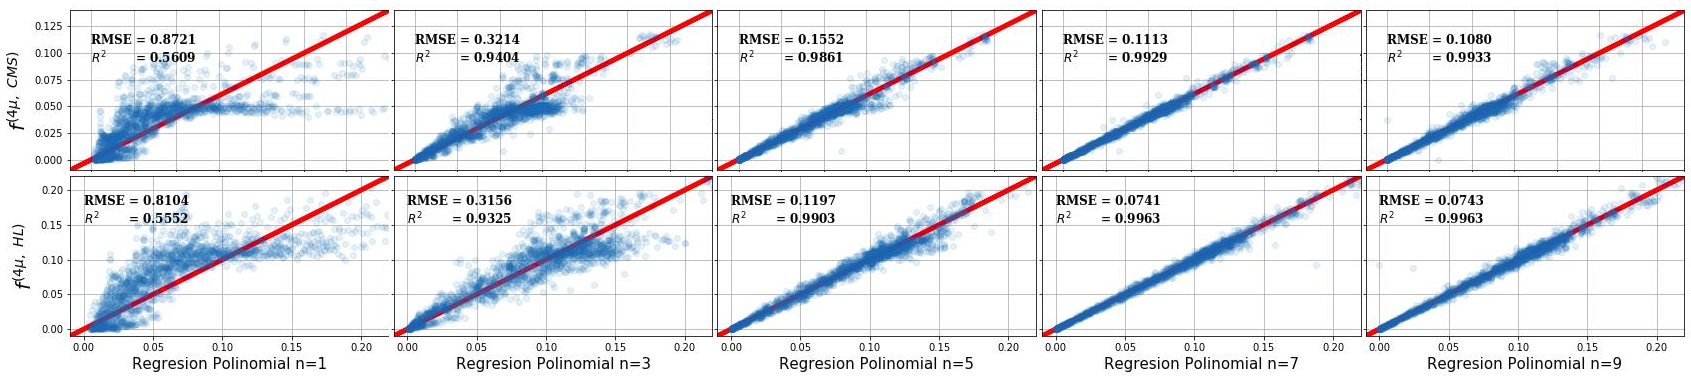
\includegraphics[width=1\textwidth]{Imag/regresionlineal.png}
\caption{Resultados del ajuste de correlaci\'on para la regresi\'on polinomial.}
\end{figure}
\end{frame}



\begin{frame}{Eficiencia para fot\'on oscuro. Regresi\'on.}
2- M\'etodo de regresi\'on con machine learning, aplicaci\'on m\'odulo keras:\\
\begin{figure}
\centering
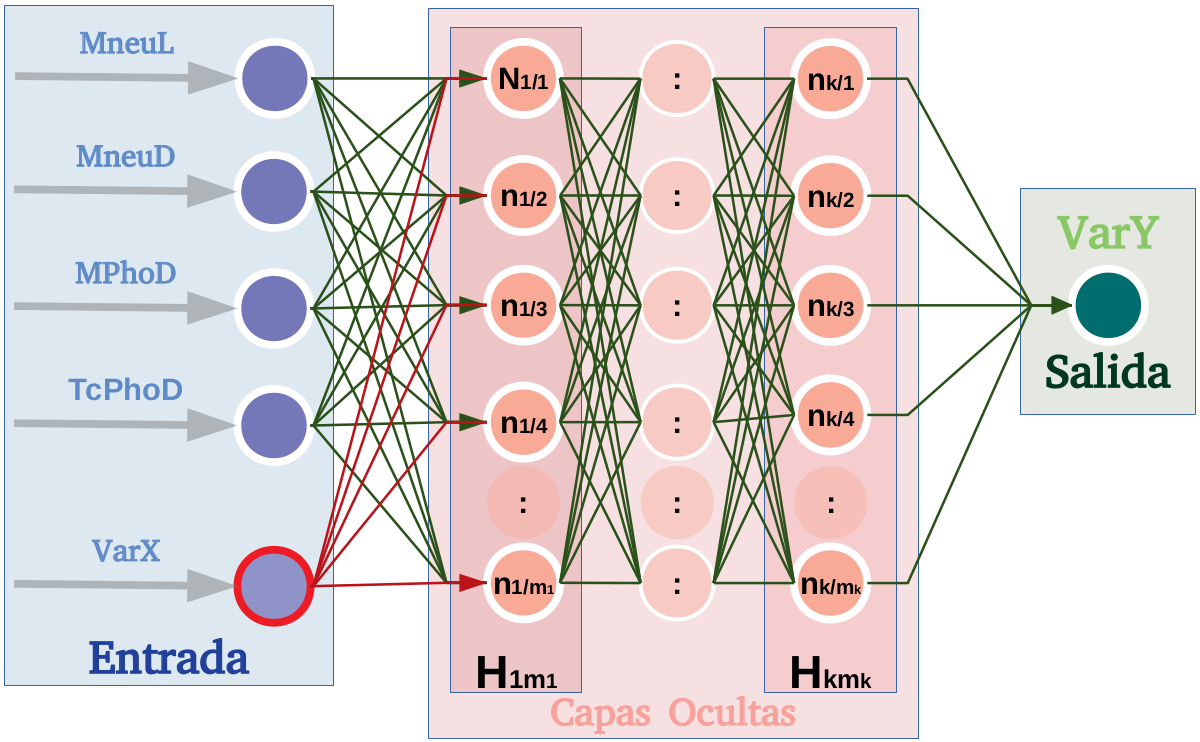
\includegraphics[width=.6\textwidth]{Imag/neuronas.png}
\caption{Diagrama de la estructura general de la red neuronal.}
\end{figure}
Para el caso de las eficiencias (VarY) este diagrama se adapta a 4 neuronas de entrada sin la variable VarX que es opcional. 
\end{frame}


\begin{frame}{Eficiencia para fot\'on oscuro. Regresi\'on.}
2- M\'etodo de regresi\'on con machine learning, aplicaci\'on m\'odulo keras:\\
Resultados y comparaci\'on:
\begin{figure}
\centering
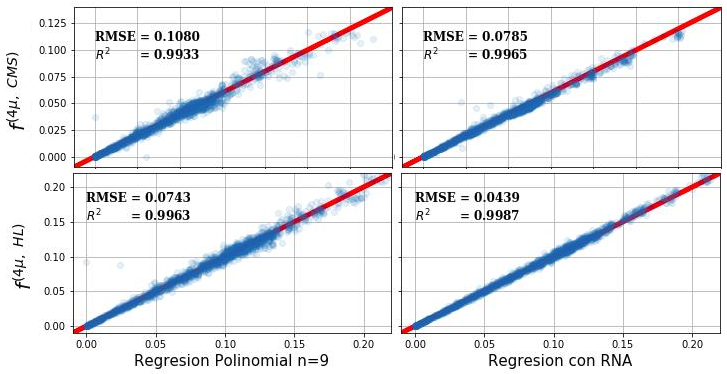
\includegraphics[width=1\textwidth]{Imag/regresion2.png}
\caption{Comparaci\'on entre los m\'etodos de regresi\'on.}
\end{figure}

\end{frame}


\begin{frame}{Etapa de Alta luminosidad para el Gran Colisionador de Hadrones}
    \begin{itemize}
        \item El Gran Colisionador de Hadrones junto con sus experimentos principales estan en una etapa de actualizacion en preparacion para la etapa de alta luminosidad (2025-2035) 
        \item En particular para la deteccion de muones se instalaran una serie de nuevos detectores que ampliaran el rango de deteccion, muy en particular para la region de pseudo-rapidez ($2.4<|\eta|<3.0$) como se muestra en el la imagen
        \item Estos nuevos detectores permitiran la identificacion de muones en esta region, y aumentaran la probabilidad de detectar se\~nales como los fotones oscuros
    \end{itemize}
\end{frame}



\begin{frame}{Actualizaci\'on del sistema de muones en el HL-LHC}

\begin{itemize}
\item La actualizaci\'on de basa en la instalaci\'on de nuevos detectores de muones 
\item Dicha detecci\'on amplia el rango de b\'usqueda para la posible detecci\'on de muones provenientes del fot\'on oscuro y otros modelos de fisica mas alla del modelo est\'andar
\end{itemize}

\begin{figure}
\centering
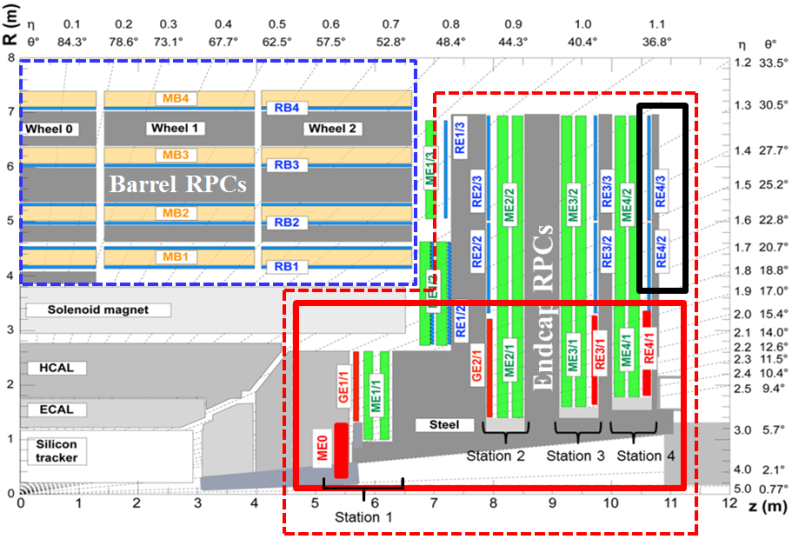
\includegraphics[width=.6\textwidth]{Imag/muon_phase-2.png}
\caption{Actualizaci\'on del sistema de muones para la fase de alta luminosidad.}
\end{figure}

\end{frame}


\begin{frame}{Comparacion distribuciones detector actual vs HL-LHC}
%\color{red} Francisco aqui poner distribucion de pseudorapidez comparando el detector actual y el detector nuevo
\begin{figure}
\centering
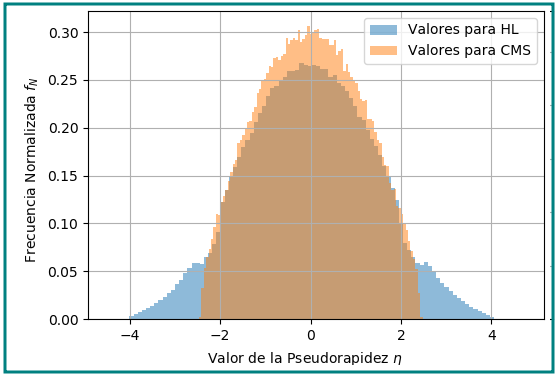
\includegraphics[width=.8\textwidth]{Imag/Datos_Eta_ALL_simple.png}
\caption{Comparar pseudorapidez.}
\end{figure}  
\end{frame}

\begin{frame}{Comparacion distribuciones detector actual vs HL-LHC}
\begin{figure}
\centering
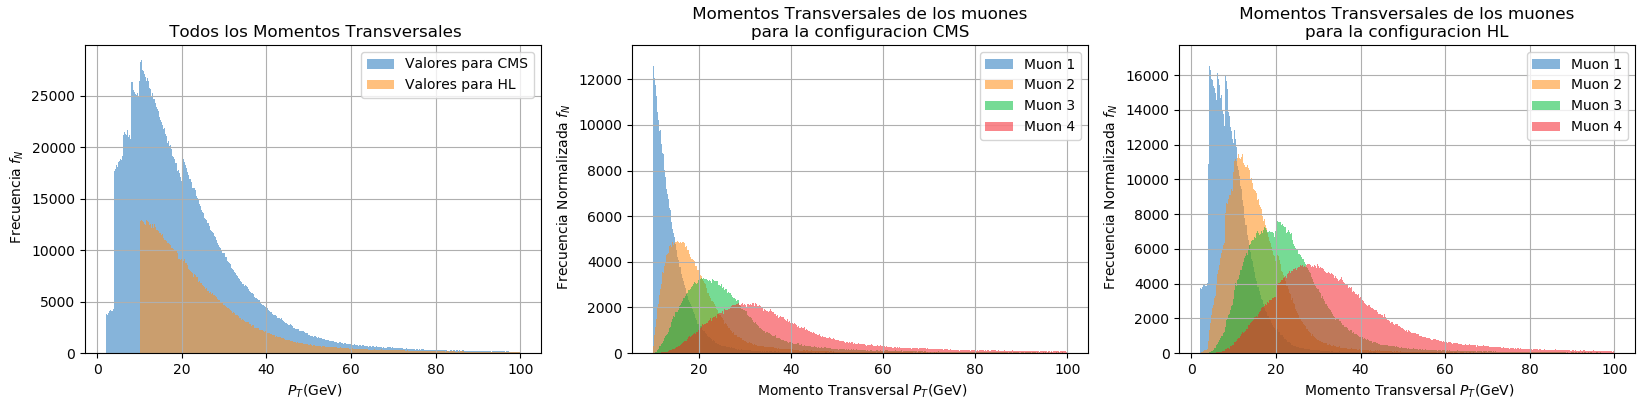
\includegraphics[width=1\textwidth]{Imag/momento1.png}
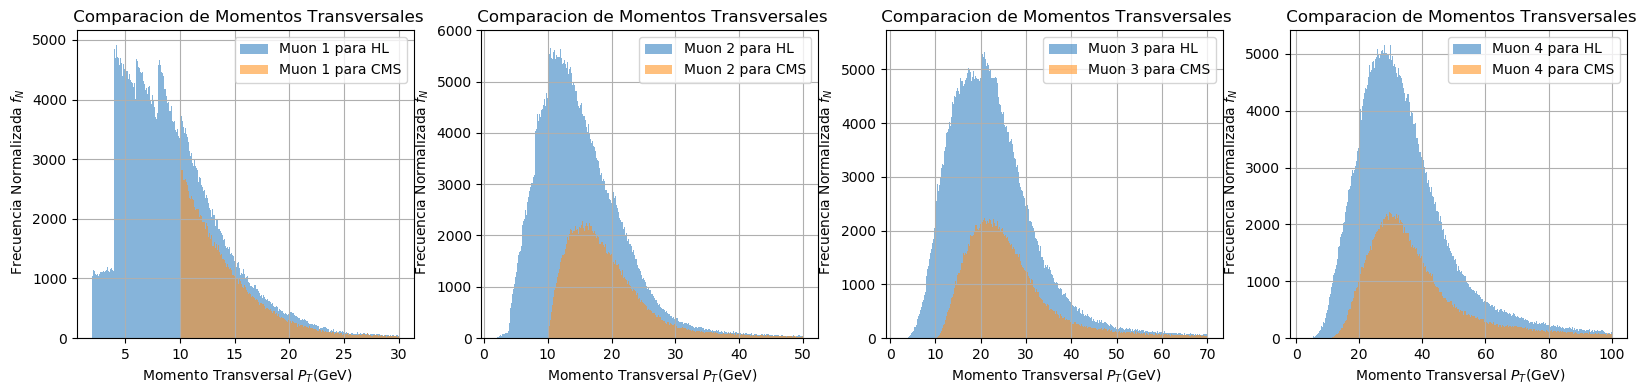
\includegraphics[width=1\textwidth]{Imag/momento2.png}
\caption{Comparar momentos.}
\end{figure}  
\end{frame}



\begin{frame}{Comparaci\'on de eficiencias detector actual vs HL-LHC.}
    
\begin{itemize}
\item Las ventajas de las actualizaciones se ve reflejada como una aumento en la eficiencia de la se\~nal
\item La b\'usqueda del fot\'on oscuro durante el HL-LHC es uno de los objetivos fundamentales
\end{itemize}
    
\begin{figure}[h]
\centering
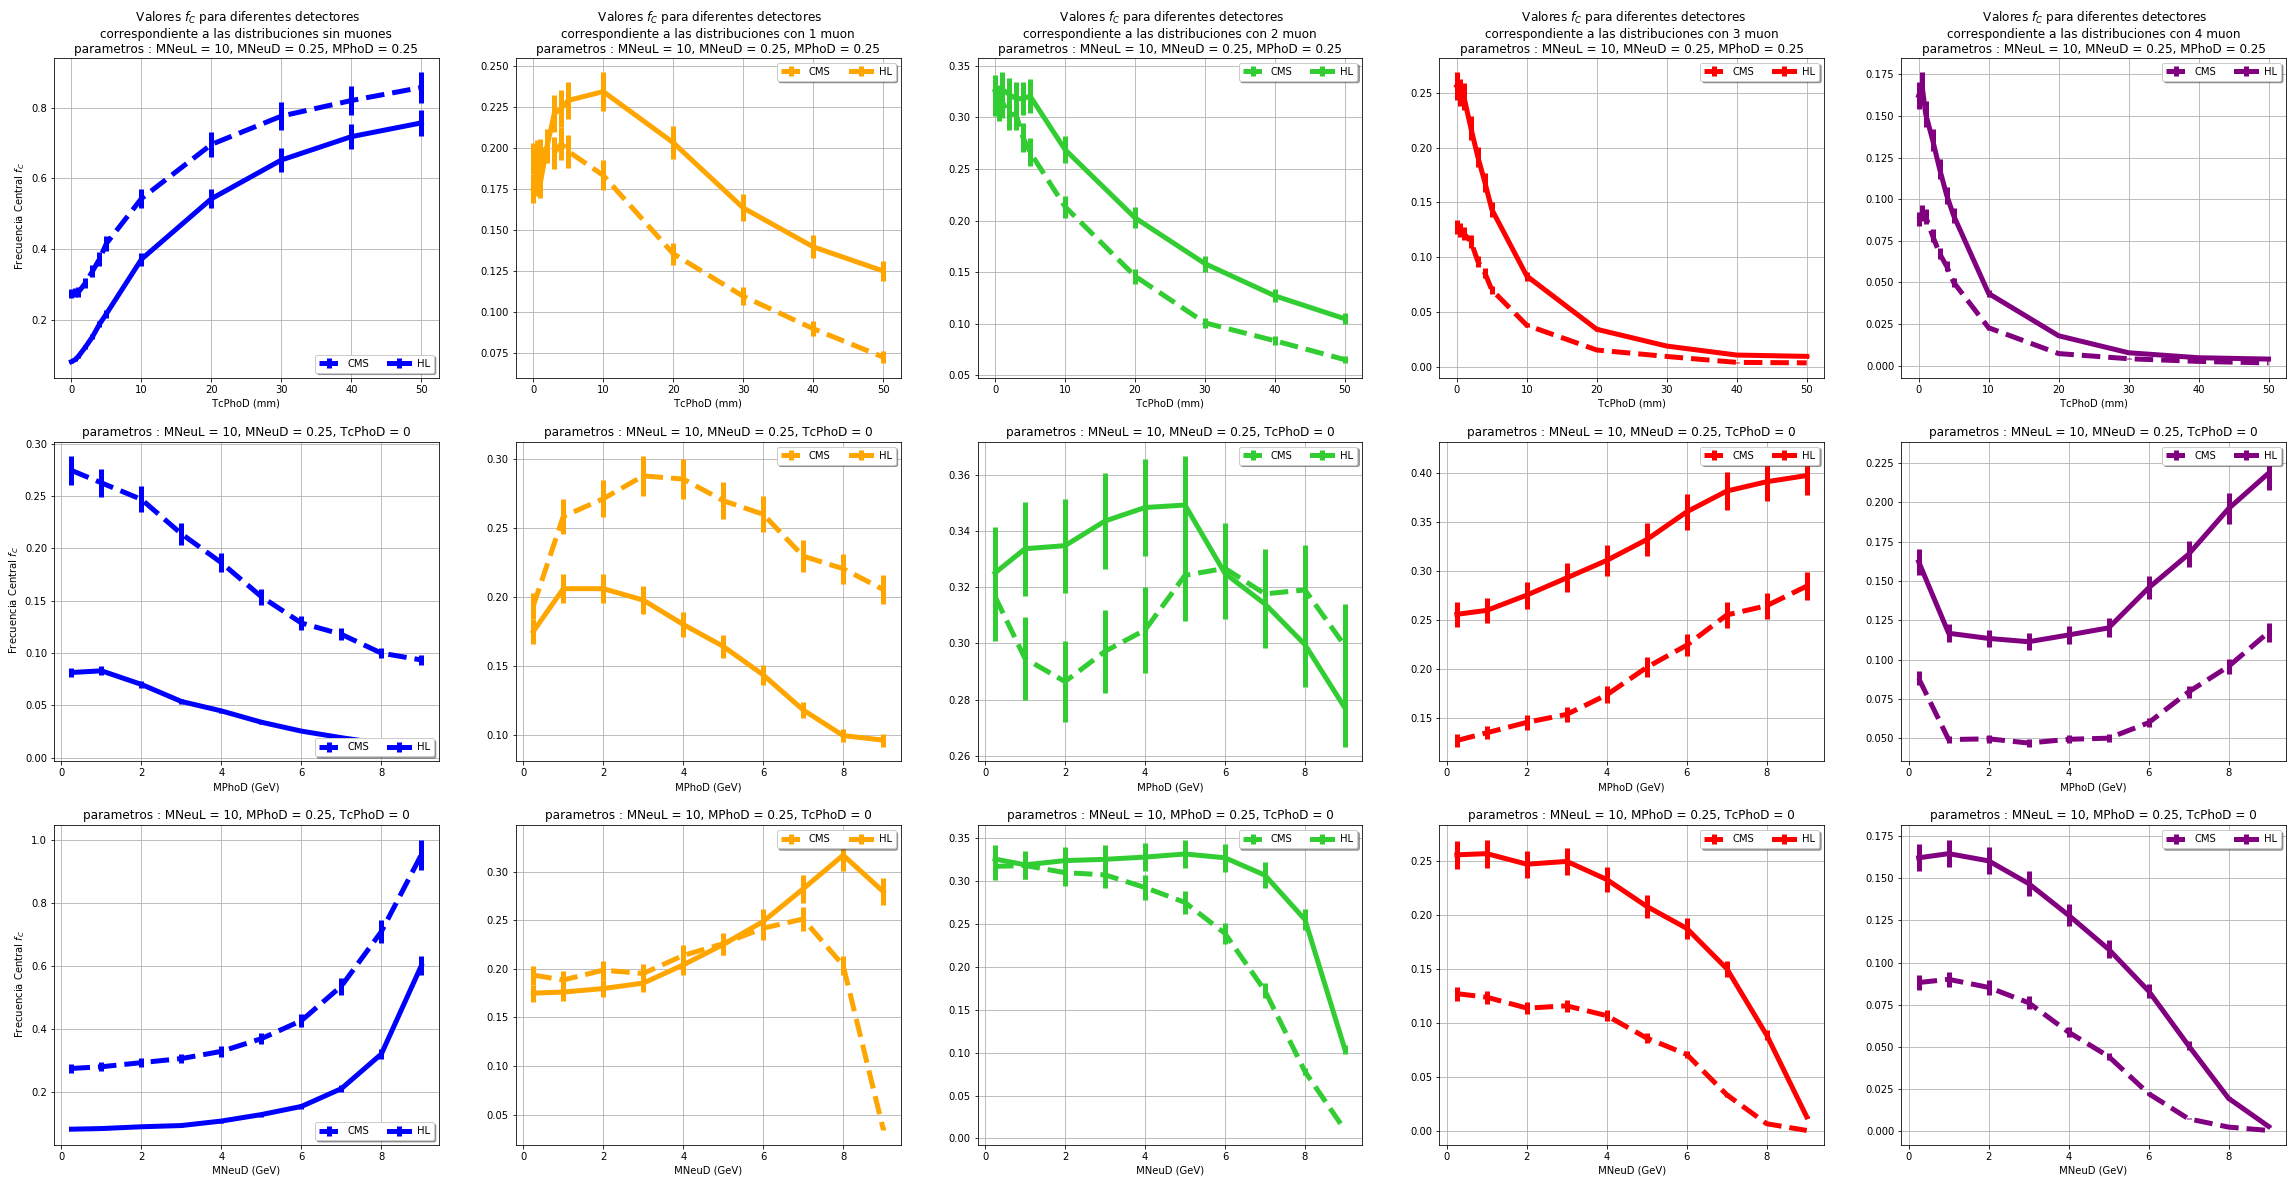
\includegraphics[width=0.7\textwidth]{Imag/Comparacion_Distribucion_Entries.png}
\caption{Comparaci\'on de eficiencias del detector actual vs HL-LHC para las diferentes muestras}
\end{figure}

\end{frame}


\begin{frame}{Comparaci\'on de eficiencias detector actual vs HL-LHC.}

\begin{itemize}
\item se logr\'a una mejor estimaci\'on de la masa.
\end{itemize}
\begin{figure}[h]
\centering
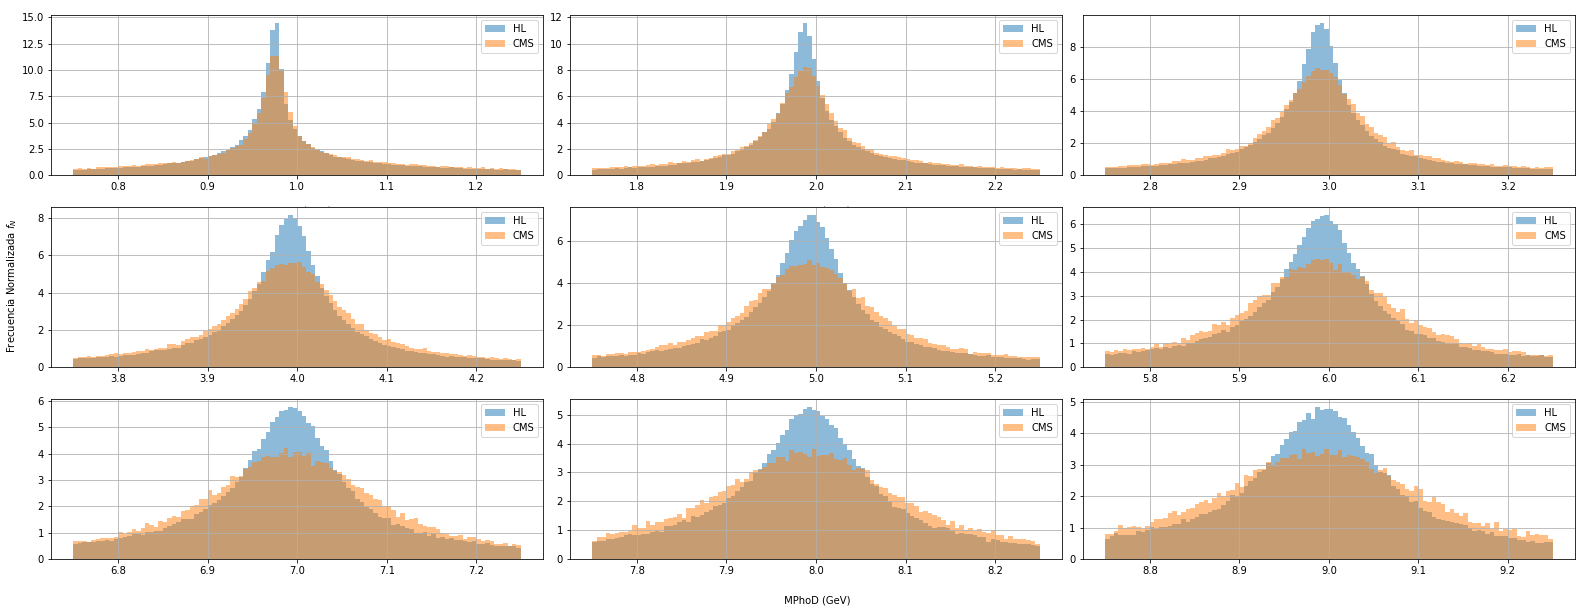
\includegraphics[width=1\textwidth]{Imag/Datos_Photon4muon_ALL.png}
\caption{Comparaci\'on de la distribuci\'on normalizada de masas del fot\'on.}
\end{figure}
\end{frame}



\begin{frame}{Resumen}
\begin{itemize}
\item Se integro el modelo Dark-SUSY en un entorno de simulaci\'on
\item Se desarrollo un entorno de simulaci\'on y an\'alisis el cual usa los recursos computacionales de la Universidad de Sonora (ACARUS) para generar resultados 
\item Se estudio a detalle la se\~nal caracteristica de los fotones oscuros
\item Se compar\'o la mejora en cuanto a eficiencia y rango de busqueda en la reconstruccion de muones del detector actual respecto a la actualizaci\'on en la etapa de alta luminosidad (HL-LHC) concluyendo que se tendr\'a en general $\sim$ 80-150\% m\'as de reconstrucciones de inter\'es para el fot\'on oscuro y un $\sim$ 12-19\% menos de errores en los valores de masa del fot\'on reconstruidos. %\color{red} Francisco poner una estimacion de este numero XXX\% \color{black} 
%de eficiencia en la b\'usqueda de esta se\~nal
\end{itemize}
  
\end{frame}



\begin{frame}{Siguientes Pasos}
\begin{itemize}
\item Finalizar escritura de tesis (Finales de Junio) 
\item Distribuir primer draft a  principios de Julio
\item Presentar a finales de Julio o principios de Agosto
\end{itemize}
    
\end{frame}


%\begin{frame}{What is haplotyping and why is it important?}
%  You hopefully know this after the previous three talks\dots
%\end{frame}
%
%\begin{frame}[t]{General formalization of haplotyping.}
%  \begin{block}{Inputs}
%    \begin{itemize}
%    \item A \alert{genotype matrix} $G$.
%    \item The \alert{rows} of the matrix are \alert{taxa / individuals}.
%    \item The \alert{columns} of the matrix are \alert{SNP sites /
%        characters}. 
%    \end{itemize}
%  \end{block}
%  \begin{block}{Outputs}
%    \begin{itemize}
%    \item A \alert{haplotype matrix} $H$.
%    \item Pairs of rows in $H$ \alert{explain} the rows of $G$.
%    \item The haplotypes in $H$ are \alert{biologically plausible}. 
%    \end{itemize}
%  \end{block}
%\end{frame}
%
%
%\begin{frame}[t]{Our formalization of haplotyping.}
%  \begin{block}{Inputs}
%    \begin{itemize}
%    \item A genotype matrix $G$.
%    \item The rows of the matrix are individuals / taxa.
%    \item The columns of the matrix are SNP sites / characters.
%    \item<alert@1->
%      The problem is directed: one haplotype is known.
%    \item<alert@1->
%      The input is biallelic: there are only two homozygous
%      states (0 and 1) and one heterozygous state (2).
%    \end{itemize}
%  \end{block}
%  \begin{block}{Outputs}
%    \begin{itemize}
%    \item A haplotype matrix $H$.
%    \item Pairs of rows in $H$ explain the rows of $G$.
%    \item<alert@1> The haplotypes in $H$ form a perfect phylogeny.
%    \end{itemize}
%  \end{block}
%\end{frame}
%
%
%\begin{frame}{We can do perfect phylogeny haplotyping efficiently, but
%    \dots}
%  \begin{enumerate}
%  \item \alert{Data may be missing.}
%    \begin{itemize}
%    \item This makes the problem NP-complete \dots
%    \item \dots even for very restricted cases.
%    \end{itemize}
%    \textcolor{green!50!black}{Solutions:}
%    \begin{itemize}
%    \item Additional assumption like the rich data hypothesis. 
%    \end{itemize}
%  \item \alert{No perfect phylogeny is possible.}
%    \begin{itemize}
%    \item This can be caused by chromosomal crossing-over effects.
%    \item This can be caused by incorrect data.
%    \item This can be caused by multiple mutations at the same sites.
%    \end{itemize}
%    \textcolor{green!50!black}{Solutions:}
%    \begin{itemize}
%    \item Look for phylogenetic networks.
%    \item Correct data.
%    \item<alert@1->
%       Find blocks where a perfect phylogeny is possible.
%    \end{itemize}
%  \end{enumerate}
%\end{frame}
%
%
%\subsection{The Integrated Approach}
%
%\begin{frame}{How blocks help in perfect phylogeny haplotyping.}
%  \begin{enumerate}
%  \item Partition the site set into overlapping contiguous blocks.
%  \item Compute a perfect phylogeny for each block and combine them.
%  \item Use dynamic programming for finding the partition.
%  \end{enumerate}
%
%  \begin{tikzpicture}
%    \useasboundingbox (0,-1) rectangle (10,2);
%    
%    \draw[line width=2mm,dash pattern=on 1mm off 1mm]
%      (0,1) -- (9.99,1) node[midway,above] {Genotype matrix}
%      (0,0.6666) -- (9.99,0.6666)
%      (0,0.3333) -- (9.99,0.3333)
%      (0,0) -- (9.99,0) node[midway,below] {\only<1>{no perfect phylogeny}};
%
%    \begin{scope}[xshift=-.5mm]
%      \only<2->
%      {
%        \draw[red,block]            (0,.5)   -- (3,.5)
%          node[midway,below] {perfect phylogeny};
%      }
%        
%      \only<3->
%      {
%        \draw[green!50!black,block] (2.5,.5)   -- (7,.5)
%          node[pos=0.6,below] {perfect phylogeny};
%      }
%
%      \only<4->
%      {
%        \draw[blue,block]           (6.5,.5) -- (10,.5)
%          node[pos=0.6,below] {perfect phylogeny};
%      }
%    \end{scope}
%  \end{tikzpicture}
%\end{frame}
%
%\begin{frame}{Objective of the integrated approach.}
%  \begin{enumerate}
%  \item Partition the site set into \alert{noncontiguous} blocks. 
%  \item Compute a perfect phylogeny for each block and combine them. 
%  \item<alert@1-> Compute partition while computing perfect
%    phylogenies. 
%  \end{enumerate}
%
%  \begin{tikzpicture}
%    \useasboundingbox (0,-1) rectangle (10,2);
%
%    \draw[line width=2mm,dash pattern=on 1mm off 1mm]
%      (0,1) -- (9.99,1) node[midway,above] {Genotype matrix}
%      (0,0.6666) -- (9.99,0.6666)
%      (0,0.3333) -- (9.99,0.3333)
%      (0,0) -- (9.99,0) node[midway,below] {\only<1>{no perfect phylogeny}};
%
%    \only<2->
%    {
%      \begin{scope}[xshift=-0.5mm]
%        \draw[red,block] (0,.5)   -- (3,.5) 
%          node[midway,below] {perfect phylogeny}
%                         (8,.5) -- (9,.5);
%
%        \draw[green!50!black,block]
%          (3,.5)   -- (6,.5)
%            node[pos=0.6,below] {perfect phylogeny}
%          (6.4,.5)   -- (8,.5)
%          (9,.5) -- (10,.5);
%
%        \draw[blue,block] (6,.5) -- (6.4,.5)
%          node[midway,below=5mm] {perfect phylogeny};
%      \end{scope}
%    }
%  \end{tikzpicture}
%\end{frame}
%
%
%\begin{frame}{The formal computational problem.}
%  We are interested in the computational complexity of \\
%  \alert{the function \alert{$\chi_{\operatorname{PP}}$}}:
%  \begin{itemize}
%  \item It gets genotype matrices as input.
%  \item It maps them to a number $k$.
%  \item This number is minimal such that the sites can be
%    covered by $k$ sets, each admitting a perfect phylogeny.
%    \\
%    (We call this a \alert{pp-partition}.)
%  \end{itemize}
%\end{frame}
%
%
%\section{Bad News: Hardness Results}
%
%\subsection{Hardness of PP-Partitioning of Haplotype Matrices}
%
%\begin{frame}{Finding pp-partitions of haplotype matrices.}
%  We start with a special case:
%  \begin{itemize}
%  \item The inputs $M$ are \alert{already haplotype matrices}.
%  \item The inputs $M$ \alert{do not allow a perfect phylogeny}.
%  \item What is $\chi_{\operatorname{PP}}(M)$?
%  \end{itemize}
%  \begin{example}
%    \begin{columns}
%      \column{.3\textwidth}
%      $M\colon$
%      \footnotesize
%      \begin{tabular}{cccc}
%        0 & 0 & 0 & 1 \\
%        0 & 1 & 0 & 0 \\
%        1 & 0 & 0 & 0 \\
%        0 & 1 & 0 & 0 \\
%        1 & 0 & 0 & 0 \\
%        0 & 1 & 0 & 1 \\
%        1 & 1 & 0 & 0 \\
%        0 & 0 & 1 & 0 \\
%        1 & 0 & 1 & 0
%      \end{tabular}%
%      \only<2>
%      {%
%        \begin{tikzpicture}
%          \useasboundingbox (2.9,0);
%
%          \draw [red, opacity=0.7,line width=1cm] (1.7 ,1.9) -- (1.7 ,-1.7);
%          \draw [blue,opacity=0.7,line width=5mm] (0.85,1.9) -- (0.85,-1.7)
%                                                  (2.55,1.9) -- (2.55,-1.7);
%        \end{tikzpicture}
%      }
%      \column{.6\textwidth}
%      \begin{overprint}
%        \onslide<1>
%        No perfect phylogeny is possible.
%        
%        \onslide<2>
%        \textcolor{blue!70!bg}{Perfect phylogeny}
%        
%        \textcolor{red!70!bg}{Perfect phylogeny}
%        
%        $\chi_{\operatorname{PP}}(M) = 2$.
%        
%      \end{overprint}
%    \end{columns}
%  \end{example}
%\end{frame}
%
%\begin{frame}{Bad news about pp-partitions of haplotype matrices.}
%  \begin{theorem}
%    Finding \alert{optimal pp-partition of haplotype matrices}\\
%    is equivalent to finding \alert{optimal graph colorings}.
%  \end{theorem}
%
%  \begin{proof}[Proof sketch for first direction]
%    \begin{enumerate}
%    \item Let $G$ be a graph.
%    \item Build a matrix with a column for each vertex of $G$.
%    \item For each edge of $G$ add four rows inducing\\the
%      submatrix $\left(
%        \begin{smallmatrix}
%          0 & 0 \\
%          0 & 1 \\
%          1 & 0 \\
%          1 & 1
%        \end{smallmatrix}\right)$.
%    \item The submatrix enforces that the columns lie in different
%      perfect phylogenies. \qedhere  
%    \end{enumerate}
%  \end{proof}
%\end{frame}
%
%\begin{frame}{Implications for pp-partitions of haplotype matrices.}
%  \begin{corollary}
%    If $\chi_{\operatorname{PP}}(M) = 2$ for a haplotype matrix $M$,
%    we can find an optimal pp-partition in polynomial time. 
%  \end{corollary}
%
%  \begin{corollary}
%    Computing $\chi_{\operatorname{PP}}$ for haplotype matrices is
%    \begin{itemize}
%    \item $\operatorname{NP}$-hard,
%    \item not fixed-parameter tractable, unless
%      $\operatorname{P}=\operatorname{NP}$, 
%    \item very hard to approximate.
%    \end{itemize}
%  \end{corollary}
%\end{frame}
%
%
%\subsection{Hardness of PP-Partitioning of Genotype Matrices}
%
%
%\begin{frame}{Finding pp-partitions of genotype matrices.}
%  Now comes the general case:
%  \begin{itemize}
%  \item The inputs $M$ are \alert{genotype matrices}.
%  \item The inputs $M$ \alert{do not allow a perfect phylogeny}.
%  \item What is $\chi_{\operatorname{PP}}(M)$?
%  \end{itemize}
%  \begin{example}
%    \begin{columns}
%      \column{.3\textwidth}
%      $M\colon$
%      \footnotesize
%      \begin{tabular}{cccc}
%        2 & 2 & 2 & 2 \\
%        1 & 0 & 0 & 0 \\
%        0 & 0 & 0 & 1 \\
%        0 & 0 & 1 & 0 \\
%        0 & 2 & 2 & 0 \\
%        1 & 1 & 0 & 0 
%      \end{tabular}%
%      \only<2>
%      {%
%        \begin{tikzpicture}
%          \useasboundingbox (2.9,0);
%          
%          \draw [red, opacity=0.7,line width=1cm] (1.7 ,1.3) -- (1.7 ,-1.1);
%          \draw [blue,opacity=0.7,line width=5mm] (0.85,1.3) -- (0.85,-1.1)
%                                                  (2.55,1.3) -- (2.55,-1.1);
%        \end{tikzpicture}
%      }
%      \column{.6\textwidth}
%      \begin{overprint}
%        \onslide<1>
%        No perfect phylogeny is possible.
%        
%        \onslide<2>
%        \textcolor{blue!70!bg}{Perfect phylogeny}
%        
%        \textcolor{red!70!bg}{Perfect phylogeny}
%        
%        $\chi_{\operatorname{PP}}(M) = 2$.
%        
%      \end{overprint}
%    \end{columns}
%  \end{example}
%\end{frame}
%
%
%\begin{frame}{Bad news about pp-partitions of haplotype matrices.}
%  \begin{theorem}
%    Finding \alert{optimal pp-partition of genotype matrices}
%    is at least as hard as finding \alert{optimal colorings of
%      3-uniform hypergraphs}. 
%  \end{theorem}
%
%  \begin{proof}[Proof sketch]
%    \begin{enumerate}
%    \item Let $G$ be a 3-uniform hypergraph.
%    \item Build a matrix with a column for each vertex of $G$.
%    \item For each hyperedge of $G$ add four rows inducing\\ the submatrix
%      $\left(
%        \begin{smallmatrix}
%          2 & 2 & 2 \\
%          1 & 0 & 0 \\
%          0 & 1 & 0 \\
%          0 & 0 & 1
%        \end{smallmatrix}\right)
%      $.
%    \item The submatrix enforces that the three columns do not all lie
%      in the same perfect phylogeny. \qedhere
%    \end{enumerate}
%  \end{proof}
%\end{frame}
%
%\begin{frame}{Implications for pp-partitions of genotype matrices.}
%  \begin{corollary}
%    Even if we know $\chi_{\operatorname{PP}}(M) = 2$ for a genotype matrix $M$,\\
%    finding a pp-partition of any fixed size is still
%    \begin{itemize}
%    \item $\operatorname{NP}$-hard,
%    \item not fixed-parameter tractable, unless
%      $\operatorname{P}=\operatorname{NP}$, 
%    \item very hard to approximate.
%    \end{itemize}
%  \end{corollary}
%\end{frame}
%
%
%\section{Good News: Tractability Results}
%
%\subsection{Perfect Path Phylogenies}
%
%\begin{frame}{Automatic optimal pp-partitioning is hopeless, but\dots}
%  \begin{itemize}
%  \item The hardness results are \alert{worst-case} results for\\
%    \alert{highly artificial inputs}.
%  \item \alert{Real biological data} might have special properties
%    that make the problem \alert{tractable}.
%  \item One such property is that perfect phylogenies are often
%    perfect \alert{path} phylogenies:
%
%    In HapMap data, in 70\% of the blocks where a perfect phylogeny
%    is possible a perfect path phylogeny is also possible.
%  \end{itemize}  
%\end{frame}
%
%
%\begin{frame}{Example of a perfect path phylogeny.}
%  \begin{columns}[t]
%    \column{.3\textwidth}
%    \begin{exampleblock}{Genotype matrix}
%      $G\colon$
%      \begin{tabular}{ccc}
%        A & B & C \\\hline
%        2 & 2 & 2 \\
%        0 & 2 & 0 \\
%        2 & 0 & 0 \\
%        0 & 2 & 2 
%      \end{tabular}
%    \end{exampleblock}
%
%    \column{.3\textwidth}
%    \begin{exampleblock}{Haplotype matrix}
%      $H\colon$
%      \begin{tabular}{ccc}
%        A & B & C \\\hline
%        1 & 0 & 0 \\
%        0 & 1 & 1 \\
%        0 & 0 & 0 \\
%        0 & 1 & 0 \\
%        0 & 0 & 0 \\
%        1 & 0 & 0 \\
%        0 & 0 & 0 \\
%        0 & 1 & 1 
%      \end{tabular}
%    \end{exampleblock}
%
%    \column{.4\textwidth}
%    \begin{exampleblock}{Perfect path phylogeny}
%      \begin{center}
%        \begin{tikzpicture}[auto,thick]
%          \tikzstyle{node}=%
%          [%
%            minimum size=10pt,%
%            inner sep=0pt,%
%            outer sep=0pt,%
%            ball color=example text.fg,%
%            circle%
%          ]
%        
%          \node [node] {} [->]
%            child {node [node] {} edge from parent node[swap]{A}}
%            child {node [node] {}
%              child {node [node] {} edge from parent node{C}}
%              edge from parent node{B}
%            };
%        \end{tikzpicture}
%      \end{center}
%    \end{exampleblock}
%  \end{columns}
%\end{frame}
%
%
%\begin{frame}{The modified formal computational problem.}
%  We are interested in the computational complexity of \\
%  the function $\chi_{\alert{\operatorname{PPP}}}$:
%  \begin{itemize}
%  \item It gets genotype matrices as input.
%  \item It maps them to a number $k$.
%  \item This number is minimal such that the sites can be
%    covered by $k$ sets, each admitting a perfect \alert{path} phylogeny.
%    \\
%    (We call this a ppp-partition.)
%  \end{itemize}
%\end{frame}
%
%
%
%\subsection{Tractability of PPP-Partitioning of Genotype Matrices}
%
%\begin{frame}{Good news about ppp-partitions of genotype matrices.}
%  \begin{theorem}
%    \alert{Optimal ppp-partitions of genotype matrices} can be
%    computed in \alert{polynomial time}. 
%  \end{theorem}
%  \begin{block}{Algorithm}
%    \begin{enumerate}
%    \item Build the following partial order:
%      \begin{itemize}
%      \item Can one column be above the other in a phylogeny?
%      \item Can the columns be the two children of the root of a
%        perfect path phylogeny?
%      \end{itemize}
%    \item Cover the partial order with as few compatible chain pairs 
%      as possible. 
%
%      For this, a maximal matching in a special graph needs to be
%      computed.
%    \end{enumerate}
%  \end{block}
%  \hyperlink{algorithm<1>}{\beamergotobutton{The algorithm in action}}
%  \hypertarget{return}{}
%\end{frame}
%
%\section*{Summary}
%
%\begin{frame}
%  \frametitle<presentation>{Summary}
%
%  \begin{itemize}
%  \item
%    Finding optimal pp-partitions is \alert{intractable}. 
%  \item
%    It is even intractable to find a pp-partition when \alert{just two 
%      noncontiguous  blocks are known to suffice}.
%  \item
%    For perfect \alert{path} phylogenies, optimal partitions can be
%    computed \alert{in polynomial time}.
%  \end{itemize}
%\end{frame}
%
%
%\appendix
%
%\section*{Appendix}
%
%\begin{frame}[label=algorithm]{The algorithm in action.}{Computation of
%    the partial order.}
%  \begin{columns}[t]
%    \column{.4\textwidth}
%    \begin{exampleblock}{Genotype matrix}
%      $G\colon$
%      \begin{tabular}{ccccc}
%        A & B & C & D & E \\\hline
%        2 & 2 & 2 & 2 & 2 \\
%        0 & 1 & 2 & 1 & 0 \\
%        1 & 0 & 0 & 1 & 2 \\
%        0 & 2 & 2 & 0 & 0
%      \end{tabular}
%    \end{exampleblock}
%    \column{.6\textwidth}
%    \begin{exampleblock}{Partial order}
%      \begin{tikzpicture}[node distance=15mm]
%        \tikzstyle{every node}=
%        [%
%          fill=green!50!black!20,%
%          draw=green!50!black,%
%          minimum size=7mm,%
%          circle,%
%          thick%
%        ]
%
%        \node (A) {A};
%        \node (B) [right of=A] {B};
%        \node (C) [below of=B] {C};
%        \node (D) [above of=A] {D};
%        \node (E) [below of=A] {E};
%
%        \path [thick,shorten >=1pt,-stealth'] (A) edge (E)
%                         (B) edge (C)
%                         (D) edge (A)
%                             edge[bend right] (E);
%
%        \uncover<2>{
%        \path [-,blue,thick](A) edge (B)
%                                edge (C)  
%                            (B) edge (E)
%                            (C) edge (E);}
%      \end{tikzpicture}
%
%      Partial order: \tikz[baseline] \draw[thick,-stealth'] (0pt,.5ex)
%      -- (5mm,.5ex); 
%
%      \uncover<2>{\textcolor{blue}{Compatible as children of root:
%          \tikz[baseline] \draw[thick] (0pt,.5ex) -- (5mm,.5ex);}} 
%    \end{exampleblock}
%  \end{columns}  
%\end{frame}
%
%\begin{frame}{The algorithm in action.}{The matching in the special graph.}
%  \begin{columns}[t]
%    \column{.3\textwidth}
%    \begin{exampleblock}{Partial order}
%      \begin{tikzpicture}[node distance=15mm]
%        \tikzstyle{every node}=%
%        [%
%          fill=green!50!black!20,%
%          draw=green!50!black,%
%          minimum size=8mm,%
%          circle,%
%          thick%
%        ]
%
%        \node (A)              {$A$};
%        \node (B) [right of=A] {$B$};
%        \node (C) [below of=B] {$C$};
%        \node (D) [above of=A] {$D$};
%        \node (E) [below of=A] {$E$};
%
%        \path [thick,shorten >=1pt,-stealth'] (A) edge (E)
%                         (B) edge (C)
%                         (D) edge (A)
%                             edge[bend right] (E);
%
%        \path [-,blue,thick](A) edge (B)
%                                edge (C)  
%                            (B) edge (E)
%                            (C) edge (E);
%
%        \only<3->
%        {
%          \path[very thick,shorten >=1pt,-stealth',red] (D) edge (A) (B) edge (C);
%          \path [-,red,very thick](E) edge (B);
%        }
%      \end{tikzpicture}
%    \end{exampleblock}
%    \column{.7\textwidth}
%    \begin{exampleblock}{Matching graph}
%      \begin{tikzpicture}[node distance=15mm]
%        \tikzstyle{every node}=%
%        [%
%          fill=green!50!black!20,%
%          draw=green!50!black,%
%          minimum size=8mm,%
%          circle,%
%          thick,%
%          inner sep=0pt%
%        ]
%
%        \node (A)              {$A$};
%        \node (B) [right of=A] {$B$};
%        \node (C) [below of=B] {$C$};
%        \node (D) [above of=A] {$D$};
%        \node (E) [below of=A] {$E$};
%
%        \begin{scope}[xshift=4.75cm]
%          \node (A')               {$A'$};
%          \node (B') [right of=A'] {$B'$};
%          \node (C') [below of=B'] {$C'$};
%          \node (D') [above of=A'] {$D'$};
%          \node (E') [below of=A'] {$E'$};
%        \end{scope}
%        
%        \path [thick]    (A) edge (E')
%                         (B) edge (C')
%                         (D) edge (A')
%                             edge (E');
%
%        \path [blue,thick](A') edge (B')
%                               edge (C')  
%                          (B') edge (E')
%                          (C') edge (E');
%
%        \only<2->
%        {
%          \path[very thick,red] (D) edge (A')
%                           (B) edge (C')
%                           (B') edge (E');
%        }
%      \end{tikzpicture}
%    \end{exampleblock}
%  \end{columns}
%
%  \medskip
%  \uncover<2->{A \alert{maximal matching} in the matching graph
%    \uncover<3>{induces\\ \alert{perfect path phylogenies}.}}
%
%  \hfill\hyperlink{return}{\beamerreturnbutton{Return}}
%\end{frame}

\end{document}


